\documentclass[12pt,twoside,a4paper]{etc/note}
%\documentclass[a4paper,12pt, draft]{article}
\documentclass[a4paper,12pt]{article}

%%% Работа с русским языком
\usepackage{cmap}					% поиск в PDF
\usepackage{mathtext} 				% русские буквы в формулах
\usepackage[T2A]{fontenc}			% кодировка
\usepackage[utf8]{inputenc}			% кодировка исходного текста
\usepackage[english,russian]{babel}	% локализация и переносы
\usepackage{indentfirst}            % красная строка в первом абзаце
\frenchspacing                      % равные пробелы между словами и предложениями

%%% Дополнительная работа с математикой
\usepackage{amsmath,amsfonts,amssymb,amsthm,mathtools} % пакеты AMS
\usepackage{icomma}                                    % "Умная" запятая

%%% Свои символы и команды
\usepackage{centernot} % центрированное зачеркивание символа
\usepackage{stmaryrd}  % некоторые спецсимволы

\renewcommand{\epsilon}{\ensuremath{\varepsilon}}
\renewcommand{\phi}{\ensuremath{\varphi}}
\renewcommand{\kappa}{\ensuremath{\varkappa}}
\renewcommand{\le}{\ensuremath{\leqslant}}
\renewcommand{\leq}{\ensuremath{\leqslant}}
\renewcommand{\ge}{\ensuremath{\geqslant}}
\renewcommand{\geq}{\ensuremath{\geqslant}}
\renewcommand{\emptyset}{\ensuremath{\varnothing}}

\DeclareMathOperator{\sgn}{sgn}
\DeclareMathOperator{\ke}{Ker}
\DeclareMathOperator{\im}{Im}
\DeclareMathOperator{\re}{Re}

\newcommand{\N}{\mathbb{N}}
\newcommand{\Z}{\mathbb{Z}}
\newcommand{\Q}{\mathbb{Q}}
\newcommand{\R}{\mathbb{R}}
\newcommand{\Cm}{\mathbb{C}}
\newcommand{\F}{\mathbb{F}}
\newcommand{\id}{\mathrm{id}}
\newcommand{\imp}[2]{
	(#1\,\,$\ra$\,\,#2)\,\,
}
\newcommand{\System}[1]{
	\left\{\begin{aligned}#1\end{aligned}\right.
}
\newcommand{\Root}[2]{
	\left\{\!\sqrt[#1]{#2}\right\}
}
\newcommand{\RR}{\R}
\newcommand{\NN}{\N}
\renewcommand{\subseteq}{\subset}
\newcommand{\sub}{\subset}
\newcommand{\sconstr}{\;\vert\;}
\newcommand{\thus}{\implies}

\newcommand{\defeq}{\vcentcolon= }
\newcommand{\defev}{\stackrel{\Delta}{\Longleftrightarrow}}
\newcommand{\deriv}[3][1]{%
	\ifthenelse{#1>1}{%
		\frac{\dlta^{#1} {#2}}{\dlta {#3}^{#1}}
	}{%
		\frac{\dlta {#2}}{\dlta {#3}}
	}%
}

\renewcommand\labelitemi{$\triangleright$}

\let\bs\backslash
\let\lra\Leftrightarrow
\let\ra\Rightarrow
\let\la\Leftarrow
\let\emb\hookrightarrow

%%% Перенос знаков в формулах (по Львовскому)
\newcommand{\hm}[1]{#1\nobreak\discretionary{}{\hbox{$\mathsurround=0pt #1$}}{}}

%%% Работа с картинками
\usepackage{graphicx}    % Для вставки рисунков
\setlength\fboxsep{3pt}  % Отступ рамки \fbox{} от рисунка
\setlength\fboxrule{1pt} % Толщина линий рамки \fbox{}
\usepackage{wrapfig}     % Обтекание рисунков текстом

%%% Работа с таблицами
\usepackage{array,tabularx,tabulary,booktabs} % Дополнительная работа с таблицами
\usepackage{longtable}                        % Длинные таблицы
\usepackage{multirow}                         % Слияние строк в таблице

%%% Теоремы
\theoremstyle{plain}
\newtheorem{theorem}{Теорема}[section]
\newtheorem{lemma}{Лемма}[section]
\newtheorem{proposition}{Утверждение}[section]
\newtheorem*{exercise}{Упражнение}
\newtheorem*{problem}{Задача}

\theoremstyle{definition}
\newtheorem{definition}{Определение}[section]
\newtheorem*{corollary}{Следствие}
\newtheorem*{note}{Замечание}
\newtheorem*{reminder}{Напоминание}
\newtheorem*{example}{Пример}

\theoremstyle{remark}
\newtheorem*{solution}{Решение}

%%% Оформление страницы
\usepackage{extsizes}     % Возможность сделать 14-й шрифт
\usepackage{geometry}     % Простой способ задавать поля
\usepackage{setspace}     % Интерлиньяж
\usepackage{enumitem}     % Настройка окружений itemize и enumerate
\setlist{leftmargin=25pt} % Отступы в itemize и enumerate

\geometry{top=25mm}    % Поля сверху страницы
\geometry{bottom=30mm} % Поля снизу страницы
\geometry{left=20mm}   % Поля слева страницы
\geometry{right=20mm}  % Поля справа страницы

\setlength\parindent{15pt}        % Устанавливает длину красной строки 15pt
\linespread{1.3}                  % Коэффициент межстрочного интервала
%\setlength{\parskip}{0.5em}      % Вертикальный интервал между абзацами
%\setcounter{secnumdepth}{0}      % Отключение нумерации разделов
%\setcounter{section}{-1}         % Нумерация секций с нуля
\usepackage{multicol}			  % Для текста в нескольких колонках
\usepackage{soulutf8}             % Модификаторы начертания
\mathtoolsset{showonlyrefs=true} % показывать номера формул только у тех, у которых есть ссылки по eqref
%%% Содержаниие
\usepackage{tocloft}
\tocloftpagestyle{main}
%\setlength{\cftsecnumwidth}{2.3em}
%\renewcommand{\cftsecdotsep}{1}
%\renewcommand{\cftsecpresnum}{\hfill}
%\renewcommand{\cftsecaftersnum}{\quad}

%%% Шаблонная информация для титульного листа
\newcommand{\CourseName}{Математический анализ}
\newcommand{\FullCourseNameFirstPart}{\so{Введение в математический анализ}}
\newcommand{\SemesterNumber}{I}
\newcommand{\LecturerInitials}{Гусев Николай Анатольевич}
\newcommand{\CourseDate}{осень 2022}
\newcommand{\AuthorInitials}{Копанов Антон}
\newcommand{\AuthorInitialssecond}{Клищ Данил}
\newcommand{\VKLink}{https://vk.com/notnako}
\newcommand{\GithubLink}{https://github.com/MIPT-Group/Lectures_Tex_Club}
\newcommand{\VKLinksecond}{https://vk.com/dan.klishch}

%%% Колонтитулы
\usepackage{titleps}
\newpagestyle{main}{
	\setheadrule{0.4pt}
	\sethead{\CourseName}{}{\hyperlink{intro}{\;Назад к содержанию}}
	\setfootrule{0.4pt}                       
	\setfoot{ФПМИ МФТИ, \CourseDate}{}{\thepage} 
}
\pagestyle{main}  

%%% Нумерация уравнений
\makeatletter
\def\eqref{\@ifstar\@eqref\@@eqref}
\def\@eqref#1{\textup{\tagform@{\ref*{#1}}}}
\def\@@eqref#1{\textup{\tagform@{\ref{#1}}}}
\makeatother                      % \eqref* без гиперссылки
\numberwithin{equation}{section}  % Нумерация вида (номер_секции).(номер_уравнения)
\mathtoolsset{showonlyrefs= true} % Номера только у формул с \eqref{} в тексте.

%%% Гиперссылки
\usepackage{hyperref}
\usepackage[usenames,dvipsnames,svgnames,table,rgb]{xcolor}
\hypersetup{
	unicode=true,            % русские буквы в раздела PDF
	colorlinks=true,       	 % Цветные ссылки вместо ссылок в рамках
	linkcolor=black!15!blue, % Внутренние ссылки
	citecolor=green,         % Ссылки на библиографию
	filecolor=magenta,       % Ссылки на файлы
	urlcolor=NavyBlue,       % Ссылки на URL
}

%%% Графика
\usepackage{tikz}        % Графический пакет tikz
\usepackage{tikz-cd}     % Коммутативные диаграммы
\usepackage{tkz-euclide} % Геометрия
\usepackage{stackengine} % Многострочные тексты в картинках
\usetikzlibrary{angles, babel, quotes}
\newcommand{\RR}{\mathbb{R}}
\newcommand{\CC}{\mathbb{C}}
\newcommand{\ZZ}{\mathbb{Z}}
\newcommand{\NN}{\mathbb{N}}
\newcommand{\QQ}{\mathbb{Q}}
\newcommand{\PP}{\mathbb{P}}
\newcommand{\EE}{\mathbb{E}}
\newcommand{\DD}{\mathbb{D}}

\newcommand{\cF}{\mathcal{F}}
\newcommand{\cN}{\mathcal{N}}
\newcommand{\cL}{\mathcal{L}}
\newcommand{\cB}{\mathcal{B}}

%%% Почти всю шаблонную информацию можно менять тут
\newcommand{\CourseDate}{\the\year{}}
\newcommand{\CourseName}{Случайные процессы}
\renewcommand{\FullCourseNameFirstPart}{\so{СЛУЧАЙНЫЕ}}
\renewcommand{\FullCourseNameSecondPart}{\so{ПРОЦЕССЫ}}
\renewcommand{\SemesterNumber}{VI СЕМЕСТР}
\renewcommand{\SchoolName}{Физтех-школа: \textit{ФПМИ}}
\renewcommand{\TrackName}{Направления: \textit{ПМФ}}
\renewcommand{\LecturerInitials}{Лектор: \textit{Широбоков Максим Геннадьевич}}
% You can add up to 4 authors (AuthorA, AuthorB, AuthorC, ...)
\renewcommand{\AuthorA}
{\href{https://vk.com/smalanchuk0}{\textit{Маланчук София}}}
% \renewcommand{\AuthorB}
% {\href{https://vk.com/}{\textit{Фамилия2 Имя2}}}
% You can leave \OverleafLink or \OverleafLink empty to make them disappear from the title page, or not empty to make them appear automatically
\renewcommand{\OverleafLink}{}
\renewcommand{\GithubLink}{https://github.com/MIPT-Group/Lectures_Tex_Club}
\renewcommand{\ImageName}{logo_LTC}

\begin{document}

\maketitle
\newpage

\hypertarget{intro}{}
\tableofcontents

\begin{task}{1}
	Пусть $\mu : \F \rightarrow [0, +\infty]$ конечно аддитивна на кольце $\F$.
	\begin{enumerate}
		\item[(а)] Докажите, что если $\mu$ счетно аддитивна, то для любых $A_k \in \F$ (при $k \in \N$) если $\mu(A_1)  < + \infty$, то 
		$$
		\mu\left(\bigcap_{k=1}^{\infty}A_k\right) = \lim\limits_{n \rightarrow \infty} \left(\bigcap_{k=1}^{n}A_k\right)
		$$
		Является ли данное условие достаточным для счетной аддитивности $\mu$?
		\item[(б)] Докажите, что если для любых $A_k \in \F$ (при $k \in \N$):
		$$
		\mu\left(\bigcap_{k=1}^{\infty}A_k\right) = \lim\limits_{n \rightarrow \infty} \left(\bigcap_{k=1}^{n}A_k\right)
		$$
		То $\mu$ счетно аддитивна. \newline
		Является ли данное условие необходимым для счетной аддитивности?
	\end{enumerate}
\end{task}

\begin{solution}
	\begin{enumerate}
		\item[(а)] Пусть имеется семейство $\{A_k\}_{k\in \N} \subset \F$, и $\mu$ --- счетно аддитивна, тогда так как $\mu(A_1) < \infty$ имеем данный страшный вывод:
		\begin{multline*}
				\mu\left(\bigcap_{k=1}^{\infty}A_k\right) = \mu(A_1) - \mu\left(A_1 \setminus \bigcap_{k=1}^{\infty}A_k\right) = \mu(A_1) - \mu\left(\bigcup_{k=1}^{\infty}A_1 \setminus A_k \right) = \\ = \mu(A_1) - \lim\limits_{n \rightarrow \infty}\mu \left(\bigcup_{k=1}^{n}A_1 \setminus A_k\right)  = \mu(A_1) - \lim\limits_{n \rightarrow \infty}\mu\left(A_1 \setminus \bigcap_{k=1}^{n}A_k\right) = \\ = \lim\limits_{n \rightarrow \infty} \left[ \mu(A_1) - \mu\left( A_1 \setminus \bigcap_{k=1}^{n}A_k\right) \right] = \lim\limits_{n \rightarrow \infty}\mu\left(\bigcap_{k=1}^{n}A_k\right)
		\end{multline*}
	Данное условие не является достаточным, контрпример:
	$$
	\mu(A) := 
	\begin{cases}
		0, A\text{ --- конечно}  \\
		+\infty,\text{ иначе}
	\end{cases}
	$$
	В таком случае, $\mu$ очевидно является конечно аддитивной, однако не счетно аддитивной.
	\item[(б)]
	 Пусть теперь выполнено $\forall \{A_k\}_{k \in \N} \subset \F$: 
	 $$
	 \mu\left(\bigcap_{k=1}^{\infty}A_k\right) = \lim\limits_{n \rightarrow \infty} \left(\bigcap_{k=1}^{n}A_k\right)
	 $$
	 Докажем, что $\mu$ --- счетно аддитивна. Не умаляя общности считаем, что $\mu(\varnothing) = 0$
	 Пусть $\{A_k\}_{k \in \N} \subset \F$. Обозначим 
	 $$
	 B_n := \bigcup_{k>n} A_k
	 $$
	 Тогда $B_n \in \F$ как разность. Кроме того имеем:
	 $$
	 \bigcap_{n \in \N} B_n = \varnothing; ~ B_{n+1} \subset B_n
	 $$
	 Тогда по предположению имеем:
	 $$
	 \lim\limits_{n \rightarrow \infty} \mu\left(B_n\right) = \lim\limits_{n \rightarrow \infty}\mu\left(\bigcap_{k=1}^nB_k\right) = \mu\left(\bigcap_{k=1}^{\infty}B_k \right) = \mu(\varnothing) = 0
	 $$
	 Тогда в силу конечной аддитивности $\mu$ имеем:
	 $$
	 \mu\left(\bigcup_{k=1}^{\infty}A_k\right) = \mu\left(\bigcup_{k=1}^n A_k \right) + \mu\left(B_n\right) = \sum_{k=1}^n\mu(A_k) + \mu(B_n)
	 $$
	 Переходя в данном равенстве к пределу при $n \rightarrow \infty$, получаем:
	 $$
	 \mu\left(\bigcup_{k=1}^{\infty}A_k\right) = \sum_{k=1}^{\infty}\mu(A_k)
	 $$
	 Таким образом, $\mu$ --- счетно аддитивна.
	 Данное условие не является необходимым, действительно, рассмотрим считающую меру:
	 $$
	 \#(A) = |A|
	 $$
	 Она, очевидно, счетно аддитивна, однако рассмотрим множества 
	 $$
	 A_k := [k, +\infty] \cap \N
	 $$
	 Ясно, что 
	 $$
	 \mu\left(\bigcap_{k\in \N} A_k\right) = \mu(\varnothing) = 0
	 $$
	 Хотя $\forall n \in \N$ выполнено
	 $$
	 \mu\left(\bigcap_{k=1}^n A_k\right) = +\infty
	 $$
	 Таким образом равенство не выполняется.
	\end{enumerate}
\end{solution}
\begin{task}{2}
	Привести пример конечно-аддитивной на полукольце меры, не являющейся счетно-аддитивной
\end{task}

\begin{solution}
	Рассмотрим меру $\mu: \CP(N) \rightarrow [0, +\infty]$
	$$
	\mu(A) = 
	\begin{cases}
		0, ~|A| < +\infty \\
		+\infty, ~|A| = +\infty
	\end{cases}
	$$
	Докажем, что данная мера является конечно-аддитивной. Рассмотрим семейство $\{A_k\}_{k=1^n}$. Рассмотрим два варианта. 
	\begin{itemize}
		\item Пусть $\exists k: |A_k| = +\infty$, тогда $\mu(A_k) = +\infty$ и так как
		$$
		\left|\bigcup_{k=1}^nA_k\right| = +\infty
		$$
		То по определению $\mu$
		$$
		\mu\left(\bigcup_{k=1}^nA_k\right) = +\infty = \sum_{k=1}^{n}\mu(A_k)
		$$
		\item Пусть теперь в семействе $\{A_k\}$ все множества конечны, тогда и $\cup_{k=1}^nA_k$ --- конечно, тогда:
		$$
		\mu\left(\bigcup_{k=1}^nA_k\right) = 0 = \sum_{k=1}^n\mu(A_k)
		$$
	\end{itemize}
	Теперь, пусть $A_k = \{k\}$, тогда: 
	$$
	\mu(\bigcup_{k=1}^{\infty}A_k) = \mu(\N) = \infty
	$$
	Но
	$$
	\sum_{k=1}^{\infty}\mu(A_k) = \sum_{k=1}^{\infty} 0 = 0
	$$
	Таким образом $\mu$ является конечно-аддитивной, но не счетно-аддитивной.
	
\end{solution}
\begin{note}
	Анализ доказательства признака Дини, показывает, что необходимым и достаточным условием сходимости ряда Фурье функции $f\in L_{2\pi}$ к $S(x_0)$ в точке $x_0$ является равенство $\lim\limits_{n\to\infty}\int\limits_{0}^\delta\varphi_{x_0}(t)\sin ntd\mu(t)=0$.
\end{note}

\begin{Def}
	Будем говорить, что $f$ удовлетворяет условию Гельдера порядка $\alpha, {\alpha\in (0,1]}$, в точке $x_0$, если существуют конечные односторонние пределы $f(x_0\pm 0)$ и константы $C>0, \delta>0$, такие, что $\forall t, 0<t<\delta, |f(x_0+t)-f(x_0+0)|\leqslant Ct^\alpha,\\ {|f(x_0-t)-f(x_0-0)|\leqslant Ct^\alpha}$.
\end{Def}

\begin{Def}
	Обобщенной односторонней производной функции $f$ в точке $x_0$ называется $f_+'(x_0)=\lim\limits_{t\to+0}\frac{f(x_0+t)-f(x_0+0)}{t}, f_-'(x_0)=\lim\limits_{t\to+0}\frac{f(x_0-t)-f(x_0-0)}{t}$.
\end{Def}

\begin{prop}
	Если $f$ имеет конечное обобщенное одностороннее производное в точке $x_0$, то $f$ удовлетворяет условию Гельдера порядка 1 (условию Липшица) в точке $x_0$.
\end{prop}

\begin{linkthm}{https://youtu.be/Vp4x2iwyLe8?t=947}[Признак Липшица]
	Если $f\in L_{2\pi}$ удовлетворяет условию Гельдера порядка $\alpha$ в точке $x_0$, то тригонометрический ряд Фурье функции $f(x)$ сходится в точке $x_0$ к $\frac{f(x_0-0)+f(x_0+0)}{2}$.
\end{linkthm}
\begin{proof}
	Хотим доказать, что ряд сходится к $S(x_0)=\frac{f(x_0-0)+f(x_0+0)}{2}$. Тогда $\varphi_{x_0}(t)=\frac{(f(x_0+t)-f(x_0+0))+(f(x_0-t)-f(x_0-0))}{t}$. Для доказательства сходимости, согласно признаку Дини, мы должны доказать суммируемость этой функции на отрезке $[0, \delta]$. Понятно, что $\varphi_{x_0}$ --- измеримая функция, осталось доказать ограниченность интеграла
	\begin{multline*}
		\left|\int\limits_{0}^\delta\varphi_{x_0}(t)d\mu(t)\right|\leqslant \int\limits_{0}^\delta\frac{|f(x_0+t)-f(x_0+0)|}{t}d\mu(t)+
		\int\limits_{0}^\delta\frac{|f(x_0-t)-f(x_0-0)|}{t}d\mu(t)\leqslant\\\leqslant 2C\int\limits_{0}^\delta t^{\alpha-1}d\mu(t)=2C\int\limits_{0}^\delta t^{\alpha-1}dt=2C\frac{\delta^\alpha}{\alpha}.
	\end{multline*}
\end{proof}

\begin{corollary}
	Если функция $f\in L_{2\pi}$ дифференцируемая в точке $x_0$, то ее тригонометрический ряд Фурье сходится к $f(x_0)$ в точке $x_0$.
\end{corollary}

\begin{linklm}{https://youtu.be/Vp4x2iwyLe8?t=1417}
	Пусть \label{lemma_11.2.2} $f\in L_{2\pi}, g$ --- измеримая, $2\pi$-периодическая, ограниченная функция. Тогда коэффициенты Фурье функции $\chi(t)=f(x+t)g(t)$ стремятся к нулю, при $n\to\infty$ равномерно по $x$.
\end{linklm}

\begin{proof}
	Обозначим $w_1(\delta, F)=\sup\limits_{0\leqslant h\leqslant \delta}\int\limits_{-\pi}^\pi|F(t+h)-F(t)|d\mu(t)$ --- интегральный модуль непрерывности функции $F$. 
	\begin{multline*}
		a_n(\chi)=\frac{1}{\pi}\int\limits_{-\pi}^\pi \chi(t)\cos ntd\mu(t)=\left[\text{ замена }t=u+\frac{\pi}{n}\right]=-\frac{1}{\pi}\int\limits_{-\pi}^\pi \chi\left(u+\frac{\pi}{n}\right)\cos nud\mu(u)=\\=-\frac{1}{2\pi}\int\limits_{-\pi}^\pi\left(\chi\left(u+\frac{\pi}{n}\right)-\chi(u) \right)\cos nud\mu(u)\Rightarrow |a_n(\chi)|\leqslant \frac{1}{2\pi}w_1(\frac{\pi}{n},\chi).
	\end{multline*}
Аналогично $|b_n(\chi)|\leqslant\dfrac{1}{2\pi}w_1\left(\dfrac{\pi}{n},\chi\right)$. Значит нам необходимо доказать, что $\lim\limits_{n\to\infty}w_1(\dfrac{\pi}{n},\chi)=0$ равномерно по $x$.

Сделаем подготовку: так как $g$ --- ограниченная, то $\exists M: |g(u)|\leqslant M, \forall u$. Также по \hyperref[lemma_12.1.1]{Лемме 1} непрерывные функции всюду плотны в смысле $L_1$, то есть $f=f_1+f_2$, где $f_1\in C[-\pi,\pi]$, значит $f_1$ --- ограниченная $\exists B:|f_1(u)|\leqslant B,\forall u$, а интеграл от $f_2$ сколь угодно мал $\int\limits_{-\pi}^\pi |f_2(t)|d\mu(t)<\frac{\varepsilon}{4M}$. Оценим
\begin{multline*}
	\int\limits_{-\pi}^\pi|\chi(t+h)-\chi(t)|d\mu(t)=\int\limits_{-\pi}^\pi|f(x+t+h)g(t+h)-f(x+t)g(t)|d\mu(t)\leqslant\\ \leqslant\int\limits_{-\pi}^\pi|f(x+t+h)-f(x+t)|\cdot|g(t+h)|d\mu(t)+\int\limits_{-\pi}^\pi|f(x+t)|\cdot |g(t+h)-g(t)|d\mu(t)\leqslant\\ \leqslant[\text{замена }u=x+t, \text{пределы интегрирования не сдвигаются, т. к. интегралы}\\ \text{ по любому отрезку длины }2\pi\text{ совпадают}]\leqslant\\ \leqslant M\int\limits_{-\pi}^\pi|f(u+h)-f(u)|d\mu(u)+\int\limits_{-\pi}^\pi|f_1(x+t)|\cdot|g(t+h)-g(t)|d\mu(t)+\frac{\varepsilon}{2}\leqslant\\ \leqslant M\cdot w_1(\frac{\pi}{n},f)+B\cdot w_1(\frac{\pi}{n},g)+\frac{\varepsilon}{2}<\text{[по \hyperref[lemma_12.1.2]{Лемме 2}]}<\varepsilon
\end{multline*}
\end{proof}

\begin{linkthm}{https://youtu.be/Vp4x2iwyLe8?t=2612}[Принцип локализации Римана-Лебега]\ \\
	Если $f\in L_{2\pi}$ и тождественно равна нулю в некотором интервале $(a,b)\subset[-\pi,\pi]$, то ее тригонометрический ряд Фурье сходится к нулю равномерно на любом отрезке $[a',b']\subset(a,b)$.
\end{linkthm}

\begin{proof}
	Посмотрим
	 \begin{figure}[h]
	 	\begin{center}
	 		\begin{tikzpicture}[
	 			scale=4,
	 			axis/.style={very thick, ->, >=stealth'},
	 			important line/.style={thick},
	 			funk/.style={color=red, very thick},
	 			dashed line/.style={dashed, thin},
	 			pile/.style={thick, ->, >=stealth', shorten <=2pt, shorten
	 				>=2pt},
	 			every node/.style={color=black}
	 			]
	 			
	 			\draw[axis] (-1.,0)  -- (0.9,0) node(xline)[right] {$x$};
	 			% Lines
	 			\draw	(-.7,-0.05) node[anchor=north] {$a$};
	 			\draw	(.5,-0.05) node[anchor=north] {$b$};
	 			\draw	(.5,0.08) node[anchor=north] {$)$};
	 			\draw	(-.7,0.08) node[anchor=north] {$($};
	 			\draw	(-.4,-0.05) node[anchor=north] {$a'$};
	 			\draw	(.2,-0.05) node[anchor=north] {$b'$};
	 			\draw	(.2,0.08) node[anchor=north] {$]$};
	 			\draw	(-.4,0.08) node[anchor=north] {$[$};
	 		\end{tikzpicture}
	 	\end{center}
	 \end{figure}\\
 Заметим $(\exists \eta>0)(\forall x\in [a',b'])(\forall t, 0\leqslant |t|< \eta)\ x+t\in (a,b)$, в качестве $\eta$ можно взять $\min(a'-a, b-b')$. Построим следующую функцию $\begin{aligned}
 	\lambda (t) = \begin{cases}
 		0,\ t\in (-\eta,\eta)\\
 		1,\ t\in[-\pi,\pi]\backslash(-\eta, \eta)
 	\end{cases}
 \end{aligned}$ и сделаем ее $2\pi$-периодической.

$$S_n(f,x)=\frac{1}{\pi}\int\limits_{-\pi}^\pi f(x+t)D_n(t)d\mu(t)=\frac{1}{\pi}\int\limits_{-\pi}^\pi f(x+t)\lambda(t)D_n(t)d\mu(t),$$ действительно, если $t$ не попадает в интервал $(-\eta,\eta): \lambda(t)=1$, если же $t\in(-\eta,\eta)$, то $\lambda(t)=0$, но тогда $x+t\in(a,b)$, где $f(x+t)=0$. 
\begin{multline*}
	D_n(t)=\frac{\sin (n+\frac{1}{2})t}{2\sin\frac{t}{2}}\Rightarrow\\
	S_n(f,x)=\frac{1}{2\pi}\int\limits_{-\pi}^\pi f(x+t)\lambda(t)\ctg\frac{t}{2}\sin ntd\mu(t)+\frac{1}{2\pi}\int\limits_{-\pi}^\pi f(x+t)\lambda(t)\cos ntd\mu(t)\overset{\text{Л. 2}}{\rightrightarrows}0, n\to\infty.
\end{multline*}
Функция $g(t)=\lambda(t)\ctg\frac{t}{2}$ --- ограниченная, измеримая, $2\pi$-периодическая, так как при $t\in(-\eta,\eta): \lambda(t)=0$, а вне $(-\eta,\eta): \ctg\frac{t}{2}$ --- ограниченная фукнция. $f$ по условию из $L_{2\pi}$. Тогда применяя \hyperref[lemma_11.2.2]{Лемму 2}, получаем, что первое слагаемое представляет собой коэффициент Фурье, который стремится равномерно по $x$ к нулю, аналогично со вторым слагаемым.
\end{proof}

\begin{corollary}
	Если $f_1$ и $f_2\in L_{2\pi}$ и $f_1\equiv f_2$ на $(a,b)$, то тригонометрические ряды Фурье равномерно равносходятся на любом отрезке $[a',b']\subset (a,b)$.
\end{corollary}

\begin{linkthm}{https://youtu.be/Vp4x2iwyLe8?t=3551}[Признак Жордана]\ \\
	Если $f \in L_{2\pi}$ и является функцией ограниченной вариации на $[a,b]$, то тригонометрический ряд Фурье $f$ сходится к $f(x_0)$ в каждой точке $x_0\in [a,b]$ непрерывности функции $f(x)$ и к $\frac{f(x_0+0)+f(x_0-0)}{2}$ в каждой точке разрыва $x_0\in[a,b]$ функции $f(x)$. Если, кроме того, $f$ непрерывна на $[a,b]$, то тригонометрический ряд Фурье функции $f$ сходится к ней равномерно на любом отрезке $[a',b']\subset(a,b)$.
\end{linkthm}

\begin{proof}
	Любая функция ограниченной вариации на отрезке $[a,b]$ представима в виде $f=f_1-f_2$, где $f_1,f_2$ --- неубывающие функции на отрезке $[a,b]$. И тригонометрический ряд Фурье от разности функций равен разности из тригонометрических рядов Фурье. Значит достаточно доказать утверждение признака Жордана только для неубывающей функции на отрезке $[a,b]$. По замечанию к признаку Дини, достаточно доказать, что $\lim\limits_{n\to\infty}\int\limits_0^\delta\varphi_{x_0}(t)\sin ntd\mu(t)=0$, где $\varphi_{x_0}(t)=\frac{f(x_0+t)-f(x_0-t)-f(x_0+0)-f(x_0-0)}{t}$. Так как $\varphi_{x_0}$ представляется в виде разности двух похожих частей, то докажем только, что $\lim\limits_{n\to\infty}\int\limits_0^\delta \frac{f(x_0+t)-f(x_0+0)}{t} \sin ntd\mu(t)=0$.
	
	Начнем с того, что ${\exists\delta_1, 0<\delta_1<\delta:0\leqslant f(x_0+\delta_1)- f(x_0+0)<\varepsilon}$, так как $f(x_0+0)$ --- это односторонний предел $f(x_0+t)$. Так как функция неубывающая, то перейдем к интегралу Римана и оценим $\int\limits_0^{\delta_1}\frac{f(x_0+t)-f(x_0+0)}{t}\sin ntdt=[\text{вторая теорема о среднем для интеграла Римана}]=f(x_0+\delta_1)-f(x_0+0)\int\limits_{\delta_2}^{\delta_1}\frac{\sin nt}{t}dt$, где $0<\delta_2<\delta_1$. Мы знаем, что $\int\limits_0^{+\infty}\frac{\sin t}{t}dt$ сходится и обозначив $G(v)=\int\limits_{0}^v\frac{\sin t}{t}dt\Rightarrow G(v)$ ограничена, то есть $\left|\int\limits_0^v\frac{\sin t}{t}dt\right|\leqslant C$, а значит $\left|\int\limits_0^A\frac{\sin nt}{t}dt\right|=[u:=nt]=\left|\int\limits_0^{nA}\frac{\sin u}{u}du\right|\leqslant C$, где $C$ не зависит от $A$. Тогда $\left|f(x_0+\delta_1)-f(x_0+0)\int\limits_{\delta_2}^{\delta_1}\frac{\sin nt}{t}dt\right|\leqslant 2\varepsilon C$.
	
	Итого $\int\limits_0^\delta \frac{f(x_0+t)-f(x_0+0)}{t} \sin ntd\mu(t)=\int\limits_0^{\delta_1} \frac{f(x_0+t)-f(x_0+0)}{t} \sin ntd\mu(t)+\int\limits_{\delta_1}^{\delta_2} \frac{f(x_0+t)-f(x_0+0)}{t} \sin ntd\mu(t)$, первый интеграл мы оценили сверху $2\varepsilon C$, для второго интеграла применяем теорему Римана об осцилляции.
	
	Докажем равномерную сходимость на отрезке $[a',b']$ TODO
\end{proof}























\newpage
\lecture{4}{Произведения сигма-алгебр.}

\begin{definition}
    \label{lect4:def:mult}
    Пусть $X,\,Y,\,Z$~--- множества, $\CE\subset \CP(X),\, \F\subset\CP(Y),\, \CG\subset \CP(Z)$.
    \begin{align*}
        P_{\CE,\,\F}        & := \{A\times B\ \vert\ A\in\CE,\,B\in\F \}                   \\
        P_{\CE,\,\F,\, \CG} & := \{A\times B\times C\ \vert\ A\in\CE,\,B\in\F,\,C\in\CG \}
    \end{align*}
\end{definition}

\begin{definition}
    Если $\CE,\,\F$ и $\CG$~--- $\sigma$"=алгебры, то
    \begin{align*}
        \CE\otimes\F           & :=\sigma(P_{\CE,\,\F})        \\
        \CE\otimes\F\otimes\CG & :=\sigma(P_{\CE,\,\F,\,\CG}),
    \end{align*}
    называется \mdef{произведением сигма-алгебр} $\CE$ и $\F$, и $\CE,\, \F$ и $\CG$ соответственно.
\end{definition}

Докажем некоторые свойства произведения сигма-алгебр.

\begin{claim}
    Если $\CE,\,\F,\,\CG$~--- $\sigma$"=алгебры, то
    \[
        (\CE\otimes\F)\otimes\CG=\CE\otimes(\F\otimes\CG)=\CE\otimes\F\otimes\CG.
    \]

    \begin{proof}
        Докажем, что $(\CE\otimes\F)\otimes\CG=\CE\otimes\F\otimes\CG$.
        По определению:
        \begin{align}
            (\CE\otimes\F)\otimes\CG & =\sigma(\{A\times B\ \vert\ A\in\CE\otimes\F,\, B\in\CG\}),\label{lect4:efg} \\
            \CE\otimes\F             & =\sigma(\{M\times N\ \vert\ M\in\CE,\, N\in\F\}).
        \end{align}
        Откуда следует, что $\forall M\in\CE,\, N\in\F$ выполнено $M\times N\in\CE\otimes\F$.
        Теперь подставим вместо $A$ в формуле \eqref{lect4:efg} $M\times N$. Получим
        $\forall B\in\CG:\ M\times N\times B\in(\CE\otimes\F)\otimes \CG$. То есть доказано вложение
        $P_{\CE,\,\F,\,\CG}\subset (\CE\otimes\F)\otimes \CG$, а это и означает, что
        $\CE\otimes\F\otimes\CG\subset (\CE\otimes\F)\otimes \CG$, так как слева и справа сигма-алгебры,
        содержащие $P_{\CE,\,\F,\,\CG}$, но слева по определению минимальная по вложению сигма-алгебра.

        Осталось доказать вложение в обратную сторону. Сначала докажем, что
        \[
            \{A\times B\ \vert\ A\in\CE\otimes\F,\, B\in\CG\}\subset\CE\otimes\F\otimes\CG.
        \]
        Из этого сразу будет следовать и вложение сигма-алгебр (снова в силу минимальности по вложению).
        Обозначим $\CM=\CE\otimes\F\otimes\CG$.
        Зафиксируем $B\in\CG$. Нужно доказать, что $A\times B\in\CM$ для $\forall A\in\CE\otimes\F$.
        Рассмотрим множество $Q$, состоящее из всех $A$, обладающих таким свойством, то есть
        \[
            Q=\{A\in\CE\otimes\F\ \vert\ A\times B\in\CM\}.
        \]
        Заметим, что $Q$ является $\sigma$"=алгеброй:
        \begin{enumerate}[label=\arabic*\degree.]
            \item $\varnothing\in Q$.
            \item Так как $A\subset X\times Y$ (смотри определение \ref{lect4:def:mult}),
                  $A\in Q\Rightarrow A^C\times B=(X\times Y\times B)\setminus (A\times B)\in\CM\Rightarrow A^C\in Q$.
            \item Аналогично для объединения: $\{A_n\}_{n\in\N},\, A_n\in Q$:
                  \[
                      \left(\bigcup_{n=1}^{\infty}A_n\right)\times B=\bigcup_{n=1}^{\infty}\left(A_n\times B\right)\in\CM
                      \Rightarrow\bigcup_{n=1}^{\infty}A_n\in Q.
                  \]
        \end{enumerate}

        С другой стороны, $P_{\CE,\, \F}\subset Q$, в самом деле, если $A=E\times F$, где $E\in\CE$, $F\in\F$, то
        $A\times B = E\times F\times B\in \CM$.
        Тогда $\CE\otimes\F\subset Q$, потому что $Q$~--- $\sigma$"=алгебра.

        Аналогично доказывается, что $\CE\otimes(\F\otimes\CG)=\CE\otimes\F\otimes\CG$, откуда и следует вся
        цепочка равенств.

    \end{proof}
\end{claim}

\subsection{Сечения множеств.}

\begin{figure}[!ht]
    \centering
    

\tikzset{every picture/.style={line width=0.75pt}} %set default line width to 0.75pt        

\begin{tikzpicture}[x=0.75pt,y=0.75pt,yscale=-1,xscale=1]
%uncomment if require: \path (0,300); %set diagram left start at 0, and has height of 300

%Straight Lines [id:da007415503180838279] 
\draw    (40,269.75) -- (40.49,33.25) ;
\draw [shift={(40.5,30.25)}, rotate = 450.12] [fill={rgb, 255:red, 0; green, 0; blue, 0 }  ][line width=0.08]  [draw opacity=0] (8.93,-4.29) -- (0,0) -- (8.93,4.29) -- cycle    ;
%Straight Lines [id:da9081056651069428] 
\draw    (21,250.25) -- (315.5,250.25) ;
\draw [shift={(318.5,250.25)}, rotate = 180] [fill={rgb, 255:red, 0; green, 0; blue, 0 }  ][line width=0.08]  [draw opacity=0] (8.93,-4.29) -- (0,0) -- (8.93,4.29) -- cycle    ;
%Shape: Polygon Curved [id:ds20201874795725505] 
\draw   (127,102) .. controls (146,84.25) and (196,86.75) .. (217,102) .. controls (238,117.25) and (254.5,131.25) .. (217,162) .. controls (179.5,192.75) and (147,192) .. (127,162) .. controls (107,132) and (108,119.75) .. (127,102) -- cycle ;
%Straight Lines [id:da9198409961373268] 
\draw    (151.5,31.25) -- (150.5,269.25) ;
%Straight Lines [id:da35659363774484776] 
\draw    (19,150.25) -- (301,150.75) ;
%Straight Lines [id:da568792556674983] 
\draw [color={rgb, 255:red, 189; green, 16; blue, 224 }  ,draw opacity=1 ] [dash pattern={on 0.84pt off 2.51pt}]  (40,90.75) -- (151,90.75) ;
%Straight Lines [id:da1699801002145609] 
\draw [color={rgb, 255:red, 189; green, 16; blue, 224 }  ,draw opacity=1 ][line width=2.25]    (151,90.75) -- (151,182.25) ;
%Straight Lines [id:da9976895793729914] 
\draw [color={rgb, 255:red, 189; green, 16; blue, 224 }  ,draw opacity=1 ] [dash pattern={on 0.84pt off 2.51pt}]  (40,182.25) -- (151,182.25) ;
%Straight Lines [id:da3185381303928254] 
\draw [color={rgb, 255:red, 189; green, 16; blue, 224 }  ,draw opacity=1 ][line width=2.25]    (40,90.75) -- (40,182.25) ;
%Straight Lines [id:da1907903601676899] 
\draw [color={rgb, 255:red, 74; green, 144; blue, 226 }  ,draw opacity=1 ] [dash pattern={on 0.84pt off 2.51pt}]  (119,150.25) -- (119.5,250.25) ;
%Straight Lines [id:da5654486602006288] 
\draw [color={rgb, 255:red, 74; green, 144; blue, 226 }  ,draw opacity=1 ] [dash pattern={on 0.84pt off 2.51pt}]  (229.5,151.25) -- (230,251.25) ;
%Straight Lines [id:da8454568946841972] 
\draw [color={rgb, 255:red, 74; green, 144; blue, 226 }  ,draw opacity=1 ][line width=2.25]    (119,150.25) -- (229.5,151.25) ;
%Straight Lines [id:da8212837531494144] 
\draw [color={rgb, 255:red, 74; green, 144; blue, 226 }  ,draw opacity=1 ][line width=2.25]    (119.5,250.25) -- (230,251.25) ;

% Text Node
\draw (52,29) node [anchor=north west][inner sep=0.75pt]   [align=left] {$\displaystyle Y$};
% Text Node
\draw (294.5,253) node [anchor=north west][inner sep=0.75pt]   [align=left] {$\displaystyle X$};
% Text Node
\draw (154.5,227) node [anchor=north west][inner sep=0.75pt]   [align=left] {$\displaystyle x$};
% Text Node
\draw (22,128.5) node [anchor=north west][inner sep=0.75pt]   [align=left] {$\displaystyle y$};
% Text Node
\draw (40.75,97.5) node [anchor=north west][inner sep=0.75pt]   [align=left] {$\displaystyle \textcolor[rgb]{0.74,0.06,0.88}{E_{x}}$};
% Text Node
\draw (195,251.5) node [anchor=north west][inner sep=0.75pt]   [align=left] {$\displaystyle \textcolor[rgb]{0.29,0.56,0.89}{E_{y}}$};
% Text Node
\draw (216,76) node [anchor=north west][inner sep=0.75pt]   [align=left] {$\displaystyle E\in X\times Y$};


\end{tikzpicture}

    \caption{Множество $E$.}
    \label{lect4:fig:mult}
\end{figure}

\begin{definition}
    Пусть $E\in X\times Y,\, x\in X,\, y\in Y$. 
    \begin{align*}
        E_x&:=\{y\in Y:\ (x,\, y)\in E\}\\
        E^y&:=\{x\in X:\ (x,\, y)\in E\}
    \end{align*}
    Для лучшего понимания смотри рисунок \ref{lect4:fig:mult}. Будем такие конструкции называть \mdef{вертикальными 
    и горизонтальными сечениями} соответственно.
\end{definition}

\begin{remark}
    Легко заметить пару свойств введенных понятий:
    \begin{enumerate}[label=\arabic*\degree.]
        \item $(E^C)_x = \{y\in Y:\ (x,\, y)\notin E\}=(E_x)^C.$
        \item Если $\{E_n\}_{n\in\N}:\ E_n\subset X\times Y$, то 
        $\left(\bigcup\limits_{n=1}^{\infty}E_n\right)_x=\bigcup\limits_{n=1}^{\infty}\left(E_n\right)_x$
        \item Если $\{E_n\}_{n\in\N}:\ E_n\subset X\times Y$, то 
        $\left(\bigcap\limits_{n=1}^{\infty}E_n\right)_x=\bigcap\limits_{n=1}^{\infty}\left(E_n\right)_x$
    \end{enumerate}
    И аналогично для горизонтальных сечений.
\end{remark}

Зададимся следующим вопросом. Верно ли, что $E_x\in\F$ и $E^y\in\CG$, если $E\in\CE\otimes\F$?

\begin{theorem}
    Пусть $\CE\in\CP(X)$ и $\F\in\CP(Y)$~--- $\sigma$"=алгебры. Тогда $\forall E\in\CE\otimes\F\ \forall x\in X\ \forall y\in Y$ 
    выполнено $E_x\in\F$ и $E^y\in\CE$.

    \begin{proof}
        Докажем только, $E_x\in\F$ (вторая вложенность будет доказываться аналогично). 
        Пусть $\CH = \{E\in\CE\otimes\F:\ E_x\in\F\}$. Заметим, что $\CH$~--- $\pi$"=система:
        если $E,\, F\in\CH$, то в силу замечания имеем $(E\cap F)_x=E_x\cap F_x\in\F$. 
        
        Докажем, что $\CH$~--- еще и $\lambda$"=система (то есть $\sigma$"=алгебра). Легко видеть, что $\varnothing\in\CH$.
        Рассмотрим $\{E_n\in\CH\}_{n\in\N}:\ E_i\cap E_j=\varnothing,\ \forall i\neq j$. Пусть тогда
        $E:=\bigsqcup\limits_{n=1}^{\infty}E_k$. Аналогично, 
        \[
            E_x=\bigsqcup_{n=1}^{\infty}(E_k)_x\in\F\text{, так как } \F\text{~--- $\sigma$"=алгебра ($E_{kx}\in\F$).}
        \]

        Итак, $\CH$~--- $\sigma$"=алгебра, а также $\CH\supset \{P\times Q\ \vert\ P\in\CE,\, Q\in\F\}$, 
        поэтому $\CH$ содержит и сигма-алгебру, порожденную этим множеством:
        $H\supset \sigma(\{P\times Q\ \vert\ P\in\CE,\, Q\in\F\})=\CE\otimes\F$.

    \end{proof}
\end{theorem}

\subsection{Монотонные классы.}

\begin{definition}
    Семейство $\F$ подмножества множества $X$ называется \mdef{монотонным классом}, если 
    $\forall \{E_k\}_{k\in\Z}\subset\F$ такой, что $E_k\subset E_{k+1}\ \forall k\in\Z$,
    выполнено $\bigcup\limits_{k\in\Z}E_k\in\F$ и $\bigcap\limits_{k\in\Z}E_k\in\F$.

    Простыми словами, множество замкнуто относительно объединения и пересечения последовательностей 
    вложенных множеств.
\end{definition}

\begin{theorem}[о монотонном классе]
    Пусть $\F\subset\CP(X)$~--- алгебра, $\CM\subset\CP(X)$~--- монотонный класс и $\F\subset \CM$.
    Тогда $\sigma(\F)\subset\CM$.

    \begin{remark}
        Доказательство аналогично доказательству теоремы Дынкина.
    \end{remark}
\end{theorem}

\subsection{Мера.}

\begin{definition}
    Пусть $X$~--- множество и $\F\subset\CP(X)$. Функция $\mu:\ \F\rightarrow[0,\,+\infty]$
    называется
    \begin{enumerate}
        \item \mdef{монотонной} (на $\F$), если для любых $A,\, B\in\F$ таких, что 
        $A\subset B$, выполнено $\mu(A)\leqslant \mu(B)$;

        \item \mdef{конечно-субаддитивной} (на $\F$), если для любого конечного
        семейства $\{A_k\}_{k=1}^n\subset\F$ такого, что $\bigcup\limits_{k=1}^n A_k\in\F$, 
        выполнено
        \[
            \mu\left(\bigcup_{k=1}^nA_k\right)\leqslant\sum_{k=1}^n\mu(A_k);
        \]
        
        \item \mdef{конечно-аддитивной} (на $\F$), если для любого \textbf{дизъюнктного} 
        конечного семейства $\{A_k\}_{k=1}^n\subset\F$, такого что 
        $\bigsqcup\limits_{k=1}^n A_k\in\F$ выполнено 
        \[
            \mu\left(\bigsqcup_{k=1}^nA_k\right)=\sum_{k=1}^n\mu(A_k);
        \]
        
        \item \mdef{счётно-субаддитивной} (\mdef{$\sigma$"=субаддитивной}) (на $F$), если для любого счётного семейства
        $\{A_k\}_{k\in\N}\subset\F$ такого, что $\bigcup\limits_{k=1}^{\infty} A_k\in\F$,
        выполнено 
        \[
            \mu\left(\bigcup_{k=1}^{\infty}A_k\right)\leqslant\sum_{k=1}^{\infty}\mu(A_k);
        \]
        
        \item \mdef{счётно-аддитивной} (\mdef{$\sigma$"=аддитивной}) (на $F$), если для любого \textbf{дизъюнктного} счётного
        семейства $\{A_k\}_{k\in\N}\subset\F$ выполнено
        \[
            \mu\left(\bigsqcup_{k=1}^{\infty}A_k\right)=\sum_{k=1}^{\infty}\mu(A_k);
        \]
        
        \item \mdef{конечной}, если $X\in\F$ и $\mu(X)<+\infty$;
        \item \mdef{сигма-конечной}, если существует последовательность $\{X_n\}_{n\in\N}\subset\F$
        такая, что $\mu(X_n)<+\infty$ при любом $n\in\N$ и $X=\bigcup\limits_{n=1}^{\infty}X_n$.
    \end{enumerate}
\end{definition}
\newpage
\lecture{5}{Эргодичность и стационарность}
\begin{Def}
    Пусть процесс $\left\{ X(t), \ t \in T \right\}$ второго порядка, $[a,b]
    \subseteq T$; функция $g(t)$ непрерывна на этом отрезке; задано разбиение $a
    = t_0 < t_1 < \dots < t_{n-1} < t_n = b$, $\tau_i \in [t_{i-1}, t_i)$, а
    $\Delta = \dst \min_{i \in \{1, \dots, n\}}\left| t_i-t_{i-1} \right|$
    называется его мелкостью. Тогда если существует такая случайная величина
    $\eta$, что
    \begin{align*}
      & \sum_{i=1}^n g(\tau_i)(X(t_i)-X(t_{i-1})) \tosk{^{\Delta \to 0}_{n \to \infty}} \eta, \ \EE \eta^2 < \infty
    \end{align*}
    то эта величина называется \textbf{интегралом Римана-Стилтьеса в
      среднеквадратичном смысле от $g(t)$ по процессу $X(t)$ в пределах от $a$
      до $b$} (интегралом Римана-Стилтьеса в СК от $g(t)$ по $X(t)$ от $a$ до
    $b$) и записывается как
    \begin{align*}
      & \eta = \int_a^bg(t)dX(t)
    \end{align*}
\end{Def}
\begin{theorem}
    Критерий существования интеграла Римана-Cтилтьеса в среднеквадратичном
    смысле. (без доказательства)
    \\
    \begin{align*}
      & \exists \eta = \int_a^bg(t)dX(t) \Leftrightarrow \exists \int_a^b\int_a^b g(t)g(s)d^2K_x(t,s) = \lim_{^{\Delta t \to 0, n_t \to \infty}_{\Delta s \to 0, n_s \to \infty}} \sum_{i,j=0}^{n_t,n_s}g(\tau_i)g(\sigma_j)\left( K_X(t_{i+1},s_{j+1}) - \right. \\
      & \left. - K_X(t_{i},s_{j+1}) - K_X(t_{i+1},s_{j}) + K_X(t_{i},s_{j})\right) < \infty
    \end{align*}  
\end{theorem}
\begin{Note}
    ~
    \\
    Определение интеграла Римана-Стилтьеса в СК от $g$ по $X$ обобщается на
    несобственный случай следующим образом:
    \begin{align*}
      & \int_a^\infty g(t)dX(t) = \LIM{b \to \infty} \int_a^bg(t)dX(t)
    \end{align*}
    \begin{align*}
      & \int_{-\infty}^b g(t)dX(t) = \LIM{a \to -\infty} \int_a^bg(t)dX(t)
    \end{align*}
    \begin{align*}
      & \int_{-\infty}^\infty g(t)dX(t) = \LIM{^{a\to -\infty}_{b \to \infty}} \int_a^bg(t)dX(t)
    \end{align*}
\end{Note}
\begin{problem}
    ~
    \\
    Пусть $X'(t)$~--- СК-производная $X(t)$. Найти ее матожидание и
    корреляционную функцию.
\end{problem}
\begin{solution}
    ~
    \\
    Матожидание:
    \begin{align*}
      & \EE X'(t) = \EE \LIM{\varepsilon \to 0}\left( \frac{X(t+\varepsilon) - X(t)}{\varepsilon} \right) = \lim_{\varepsilon \to 0}\EE \left( \frac{X(t+\varepsilon) - X(t)}{\varepsilon} \right) = \frac{d}{dt}\EE X(t)
    \end{align*}
    Корреляционная функция:
    \begin{align*}
      & R_{X'}(t,s) = \EE \left( \left( X'(t) - \EE X'(t) \right)\left( X'(s) - \EE X'(s) \right) \right) = \EE \ \LIM{^{\varepsilon \to 0}_{\delta \to 0}}\left( \left( \frac{X(t+\varepsilon) - X(t)}{\varepsilon} - \right. \right. \\
      & \left. \left. - \frac{m_X(t+\varepsilon) - m_X(t)}{\varepsilon} \right)\left( \frac{X(s+\delta) - X(s)}{\delta} - \frac{m_X(s+\delta) - m_X(s)}{\delta} \right) \right) = \lim_{^{\varepsilon \to 0}_{\delta \to 0}} \frac{1}{\varepsilon \delta} \cdot \\
      & \cdot \left( R_X(t+\varepsilon, s+\delta) - R_X(t+\varepsilon, s) - R_X(t, s+\delta) + R_X(t, s)\right) = \frac{\partial^2 R_X}{\partial t \partial s}
    \end{align*}
\end{solution}
Аналогично можно вывести и формулы для интеграла.
\begin{Prop}
    ~
    \\
    Если $Y(t) = X'(t)$, то
    \begin{align*}
      & \EE Y(t) = \frac{d}{dt} \EE X(t), \ R_Y(t,s) = \frac{\partial^2 R_Y(t)}{\partial t \partial s}
    \end{align*}
    Если
    \begin{align*}
      & Y(t) = \int_a^t X(\tau) d\tau
    \end{align*}
    то
    \begin{align*}
      & \EE Y(t) = \int_a^t \EE X(\tau) d\tau, \ R_Y(t,s) = \int_a^s\int_a^t R_X(\tau, \sigma) d\tau d\sigma
    \end{align*}  
\end{Prop}
\section{Эргодические процессы}
\begin{Def}
    Пусть процесс $\left\{ X(t), \ t \geq 0 \right\}$ второго порядка имеет
    постоянное математическое ожидание $m$ и интегрируем в среднеквадратичном на
    любом отрезке $[0;T]$. Рассмотрим процесс
\begin{align*}
  & \left \langle X \right \rangle_T = \frac{1}{T} \int_0^T X(t) dt, \ T \geq 0
\end{align*}
Если $\left \langle  X \right \rangle_T \tosk{T \to \infty} m$, то процесс
$X(t)$ называется \textbf{эргодическим в среднеквадратичном смысле по
  математическому ожиданию} (эргодическим в СК по $\EE$).
\end{Def}
\begin{example}
    ~
    \\
    Процесс $\dst \frac{W(t)}{t}$ является эргодическим в СК по $\EE$.
\end{example}
\begin{Def}
    Процесс $\left\{ X(t), \ t \geq 0 \right\}$ называется \textbf{эргодическим в
      среднеквадратичном смысле по дисперсии} (эргодическим в СК по $D$), если
    процесс $Y(t) = \cent{X}^2(t) = \left( X(t) - \EE X(t) \right)^2$ эргодичен в
    СК по $\EE$.
\end{Def}
\begin{Note}
    \begin{align*}
      & \frac{1}{T} \int_0^T Y(t) dt \tosk{} \EE \cent{X}^2(t) = DX(t)
    \end{align*}
\end{Note}
\begin{Def}
    Процесс $\left\{ X(t), \ t \geq 0 \right\}$ называется \textbf{эргодическим в
      среднеквадратичном смысле по корреляционной функции} (эргодическим в СК по
    $R$), если $\forall \tau$ процесс $Z_\tau(t) = \cent{X}(t)\cent{X}(t+\tau)$
    эргодичен в СК по $\EE$.
\end{Def}
\begin{Note}
    \begin{align*}
      & \frac{1}{T} \int_0^T Z_\tau(t) dt \tosk{} \EE \left( \cent{X}(t)\cent{X}(t+\tau) \right) = R_X(t,\tau)
    \end{align*}
\end{Note}
\begin{theorem}
    Критерий эргодичности по математическому ожиданию.
    \\
    Процесс $\left\{ X(t), \ t \geq 0 \right\}$ второго порядка с постоянным
    математическим ожиданием $m$ и интегрируемый в СК на любом $[0;T]$ эргодичен
    в СК по $\EE$ тогда и только тогда, когда
    \begin{align*}
      & \lim_{T \to \infty} \frac{1}{T^2}\int_0^T \int_0^T R_x(t,s) dt ds = 0
    \end{align*}
\end{theorem}
\begin{proof}
    \begin{align*}
      & \EE \left( \frac{1}{T} \int_{0}^T X(t) dt - m\right)^2 = \EE \left( \frac{1}{T}\left( X(t)dt - \int_0^T m dt \right) \right)^2 = R_{\frac{1}{T}\int_0^T X(t) dt} (T,T) = \\
      & = \frac{1}{T^2}\int_0^T \int_0^T R_X(t,s) dt ds
    \end{align*}
    В силу равенства при эргодичности в СК по $\EE$ к нулю стремится первое, а
    значит, и последнее выражение; в случае стремления последнего выражения к
    нулю к нему стремится и первое, а значит, процесс эргодичен в СК по $\EE$.
\end{proof}
\begin{theorem}
    Достаточное условие эргодичности по математическому ожиданию.
    \\
    Процесс $\left\{ X(t), \ t \geq 0 \right\}$ второго порядка с постоянным
    математическим ожиданием $m$ и интегрируемый в СК на любом $[0;T]$ эргодичен
    в СК по $\EE$, если
    \begin{align*}
      & \lim_{\left| t - s \right| \to \infty} R_X(t,s) = 0
    \end{align*}
    \begin{align*}
      & \lim_{T \to \infty} \frac{1}{T} \max_{t \in [0;T]}R_X(t,t) = 0
    \end{align*}
\end{theorem}
\begin{proof}
    ~
    \\
    Выполнение данных условий влечет:
    \begin{align*}
      & \forall \varepsilon > 0 \ \exists T_0: \ \forall T = \left| t_2-t_1 \right|\geq T_0 \hookrightarrow \left| R_X(t_1,t_2) \right| < \varepsilon
    \end{align*}
    Положим
    \begin{align*}
      & G_1 = \left\{ (t_1,t_2) \in [0;T]^2: \ \left| t_2-t_1 \right| > T_0 \right\}
    \end{align*}
    \begin{align*}
      & G_2 = \left\{ (t_1,t_2) \in [0;T]^2: \ \left| t_2-t_1 \right| \leq T_0 \right\}
    \end{align*}
    и $S_1$, $S_2$ соответственно~--- их площади. Тогда
    \begin{align*}
      & \left| \frac{1}{T^2} \int_0^T\int_0^TR_X(t_1,t_2)dt_1dt_2 \right| = \frac{1}{T^2} \left( \us{G_1}{\int\int}R_X(t_1,t_2)dt_1dt_2 + \us{G_2}{\int\int}R_X(t_1,t_2)dt_1dt_2 \right) \leq \\
      & \leq \frac{1}{T^2} \left( \left| \us{G_1}{\int\int}R_X(t_1,t_2)dt_1dt_2 \right| + \left| \us{G_2}{\int\int}R_X(t_1,t_2)dt_1dt_2 \right| \right) \leq \frac{1}{T^2} \left( \us{G_1}{\int\int}\left| R_X(t_1,t_2) \right| dt_1dt_2 + \right. \\
      & \left. + \us{G_2}{\int\int}\left| R_X(t_1,t_2) \right| dt_1dt_2 \right) \leq \frac{1}{T^2} \left( \varepsilon S_1 + \max_{G_2}\left| R_X(t_1,t_2) \right| S_2 \right) \leq \varepsilon + \frac{\dst \max_{G_2}\left| R_X(t_1,t_2) \right| S_2}{T^2} \leq \\
      & \leq \varepsilon + \frac{2T_0 \dst \max_{G_2}\left| R_X(t_1,t_2) \right|}{T} \leq \varepsilon + \frac{2T_0 \sqrt{\dst \max_{G_2} R_X(t_1,t_1)R_X(t_2,t_2)}}{T} \leq \varepsilon + \frac{2T_0 \dst \max_{t \in [0;T]} R_X(t,t)}{T} \To{T \to \infty} 0
    \end{align*}
    А такой предел указан в критерии эргодичности в СК по $\EE$.
\end{proof}
\begin{Note}
    ~
    \\
    Если у процесса дисперсия растет медленнее, чем линейно, то для эргодичности
    достаточно проверить только первое условие из достаточного.
    \\
    То же верно, если
    \begin{align*}
      & \exists c: \ \forall t \ \EE X^2(t) < c
    \end{align*}
\end{Note}
\section{Стационарные процессы.}
Стационарные процессы имеют не зависящие от времени распределения сечений,
многомерные распределения, зависящие лишь от разности моментов времени, и
описывают установившиеся во времени явления.
\begin{Def}
    Процесс $\left\{ X(t), \ t \in T \right\}$ называется \textbf{стационарным в
      узком смысле}, если все его конечномерные распределения не зависят от сдвига
    по времени на одну и ту же величину, т.~е.
    \begin{align*}
      & \forall t_1, \dots, t_n \in T, \ \forall \tau: \ t_1+\tau, \dots, t_n + \tau \in T \hookrightarrow \\
      & F_X(x_1, \dots, x_n; t_1, \dots, t_n) = F_X(x_1, \dots, x_n; t_1 + \tau, \dots, t_n+\tau)
    \end{align*}
    или, что то же самое, векторы
    \begin{align*}
      & \left[ \begin{matrix}
              X(t_1) \\
              X(t_2) \\
              \dots \\
              X(t_n)
          \end{matrix} \right], \  \left[ \begin{matrix}
              X(t_1+\tau) \\
              X(t_2+\tau) \\
              \dots \\
              X(t_n+\tau)
          \end{matrix} \right]
    \end{align*}
    одинаково распределены.
\end{Def}
\begin{example}
    ~
    \\
    Одномерное распределение:
    \begin{align*}
      F_X(x,t) = F_X(x, t + \tau) \Rightarrow \EE X(t) = m_X = const , \ D X(t) = \sigma^2 = const, \ \dots
    \end{align*}
    Все моменты постоянны во времени.
    Двумерное распределение:
    \begin{align*}
      F(x_1,x_2; t_1, t_2) = F_X(x_1, x_2; t_1 + \tau, t_2 + \tau) \Rightarrow R_X(t_1,t_2) = R_X(t_1+\tau, t_2+\tau) = R_X(0, t_2-t_1)
    \end{align*}
    Корреляционная функция зависит только от разности моментов времени.
\end{example}
\begin{Def}
    Процесс $\left\{ X(t), \ t \in T \right\}$ называется \textbf{стационарным в
      широком смысле}, если его математическое ожидание постоянно во времени, а
    корреляционная функция зависит от своих аргументов только через их разность, т.~е.
    \begin{align*}
      & \EE X(t) = m = const, \ R_X(t,s) = R(t-s)
    \end{align*}
\end{Def}
\begin{Prop}
    ~
    \\
    Если процесс второго порядка стационарен в узком смысле, то он стационарен и
    в широком смысле, но не наоборот.
\end{Prop}
\begin{Proof}
    ~
    \\
    Как было показано в примере выше, условия определения широкого смысла выполняются.
\end{Proof}
\begin{example}
    ~
    \\
    Контрпример к обратному утверждению: процесс
    \begin{align*}
      & Z(t) = X\cos t + Y \sin t, t \geq 0, \ X,Y \ \IID, \ \PP\{X = 1\} = \PP\{X = -1\} = \frac{1}{2}
    \end{align*}
    стационарен в широком, но не узком смысле.
\end{example}
\begin{theorem}
    ~
    \\
    Нормальный процесс стационарен в широком смысле тогда и только тогда, когда
    он стационарен в узком смысле.
\end{theorem}
\begin{Proof}
    ~
    \\
    Нормальный процесс является процессом второго порядка, а значит,
    необходимость очевидна.
    \\
    Пусть теперь $X(t)$ стационарен в широком смысле. Возьмем произвольное
    сечение (нормальный случайный вектор)
    \begin{align*}
      & X = \left[ \begin{matrix}
              X(t_1) \\
              \dots \\
              X(t_n)
          \end{matrix} \right] \Rightarrow \varphi_X(s) = \exp \left( is^tm - \frac{1}{2}s^TRs \right), \ s = \left( s_1, \dots, s_n \right)
    \end{align*}
    При сдвиге всех $t_i$ на одну и ту же величину $\tau$ ни $m$, ни $R$ не
    изменились, тогда и $\varphi_X(s)$ не изменится, а она задает многомерные
    распределения. Они не меняются, значит, стационарность в узком смысле
    выполняется.
\end{Proof}
\begin{Note}
    ~
    \\
    Для стационарного процесса достаточно лишь первого из условий эргодичности.
    Второе выполняется автоматически.
\end{Note}
\newpage
\lecture{6}{Теорема Каратеодори.}

\subsection{Внешняя мера Лебега. Её свойства.}

\begin{definition}
    \mdef{Внешней мерой Лебега} множества $A\subset\R^d$ называется
    \[
        m^*(A):=\inf \left\{\sum_{k=1}^{\infty}m(E_k)\ \mid\ \{E_k\}_{k=1}^{\infty}\subset K^d,\ A\subset\bigcup_{k=1}^{\infty}E_k\right\}.
    \]
\end{definition}

\begin{remark}
    Отличие от верхней меры Жордана в том, что в случае меры Лебега рассматриваются счётные, а не конечные покрытия.
\end{remark}

\begin{definition}
    Множество $E\subset\R^d$ будем называть \mdef{элементарным}, если \[E=\bigsqcup\limits_{k=1}^{\infty}E_k, \text{ где } E_k\in K^d\].
\end{definition}

\begin{remark}
    Семейство всех элементарных множеств совпадает с кольцом, порожденным $K_d$, то есть $\CR(K_d)$.
\end{remark}

\begin{claim}
    Для любых множеств $A_k\subset \R^d$ выполнено
    \[
        m^*\left(\bigcup_{k=1}^{\infty}A_k\right)\leqslant\sum_{k=1}^{\infty}m^*(A_k).
    \]

    \begin{proof}
        Пусть $A_k\subset\bigcup\limits_{l=1}^{\infty}B_{k,\,l}$, где $B_{k,\,l}$~--- клетки такие, что
        \[
            \sum_{l=1}^{\infty}B_{k,\,l}<m^*\left(A_k\right) + \dfrac{\varepsilon}{2^k}.
        \]
        Так же считаем, что $m^*(A_k)<\infty$, так как иначе утверждение очевидно. Тогда можно записать
        \begin{align*}
            \bigcup_{k=1}^{\infty}A_k\subset \bigcup_{k=1}^{\infty}\bigcup_{l=1}^{\infty}B_{k,\, l}\Rightarrow
            m^*\left(\bigcup_{k=1}^{\infty}A_k\right) & \leqslant \sum_{k=1}^{\infty}\underbrace{\sum_{l=1}^{\infty}m(B_{k,\, l})}_{<m^*(A_k)+\varepsilon/2^k}\leqslant \\
                                                      & \leqslant \sum_{k=1}^{\infty}\left(m^*(A_k)+\dfrac{\varepsilon}{2^k}\right)=
            \sum_{k=1}^{\infty}m^*(A_k)+\varepsilon.
        \end{align*}

        В силу произвольности $\varepsilon$ получаем, что
        \[
            m^*\left(\bigcup_{k=1}^{\infty}A_k\right)\leqslant \sum_{k=1}^{\infty}m^*(A_k).
        \]

    \end{proof}
\end{claim}

Зададимся вопросом, чему равна внешняя мера Лебега клетки? Легко догадаться до следующего утверждения.

\begin{claim}
    $\forall A\in K_d\quad m^*(A)=m(A)$.

    \begin{proof}
        По определению $m^*(A)\leqslant m(A)$ (инфинум суммы мер клеток, которые покрывают $A$, но $A$~--- и есть клетка, которая покрывает $A$).

        Докажем неравенство в другую сторону. Пусть $\{A_k\}_{k=1}^{\infty}\in K_d$ и $A\subset\bigcup\limits_{k=1}^{\infty}A_k$.
        Тогда $A = \bigcup\limits_{k=1}^{\infty}\left(A\cap A_k\right)$, следовательно в силу того, что клеточная мера счётно-субаддитивна, получаем
        \[
            m(A)\leqslant\sum_{k=1}^{\infty} m(A\cap A_k)\leqslant\sum_{k=1}^{\infty}m(A_k)\Rightarrow m^*(A)\geqslant m(A).
        \]

    \end{proof}
\end{claim}

То есть можно считать, что внешняя мера Лебега~--- продолжение клеточной меры, в том смысле, что это функция, у которой область определения шире,
но на области определения клеточной меры они совпадают.

\begin{definition}
    Множество $A\subset \R^d$ называется \mdef{измеримым по Лебегу}, если $\forall T\subset\R^d$:
    \[
        m^*(T)=m^*(T\cap A)+m^*(T\setminus A).
    \]
\end{definition}

Возникает желание доказать, что все такие множества образуют какое-то хорошее семейство. Сделаем это в более общем виде, то есть
не для внешней меры Лебега, а для произвольной внешней меры.

\begin{definition}
    \mdef{Внешней мерой $\nu$} на множестве $X$ называется функция $\nu:\ \CP(X)\rightarrow[o,\,+\infty]$ такая, что
    \begin{enumerate}[label=\arabic*\degree]
        \item $\nu$~--- $\sigma$"=субаддитивна,
        \item $\nu$~--- монотонна,
        \item $\nu(\varnothing)=0$.
    \end{enumerate}

    \begin{remark}
        Ясно, что внешняя мера Лебега является внешней мерой.
    \end{remark}
\end{definition}

Обобщим аналогично измеримость:

\begin{definition}
    Множество $A\subset X$ называется \mdef{$\nu$"=аддитивным}, если $\forall T\subset X$:
    \[
        \nu(T)=\nu(T\cap A)+\nu(T\setminus A).
    \]

    Множество всех $\nu$"=аддитивных множеств обозначается $\Anu$.
\end{definition}

\begin{exercise}
    Рассмотрим $\nu:\ \CP(\R)\rightarrow [0,\,+\infty]$ вида \[\nu(A)=\#\{k\in\Z:\ A\cap[k,\,k+1)\neq\varnothing\},\]
    где \[
        \# M = \begin{cases}
            n,\text{ если } |M|=n, \\
            +\infty, \text{ иначе.}
        \end{cases}
    \]

    Если $A=\{x\}$, где $x\notin\Z$, то $A\notin \Anu$, так как для $k=[x]$ и $T=[k,\,k+1)$, то $\nu(T)=\nu(A)=\nu(T\setminus A)=1$, то есть
    $\nu(T)\neq\nu(T\cap A)+\nu(T\setminus A)$.

    Можно показать, что всякое множество, являющееся объединением полуинтервалов с целочисленными концами, является и $\nu$"=аддитивным.
\end{exercise}

\begin{claim}
    \label{lect06:claim}
    Если $A_k\in\Anu$ при $k\in \overline{1,n}$ и $A_k$ попарно не пересекаются, то $\forall T\subset X$
    \[
        \nu\left(T\cap\bigsqcup_{k=1}^{n}A_k\right)=\sum_{k=1}^{n}\nu(T\cap A_k).
    \]

    \begin{proof}

        В силу того, что $A_n\in\Anu$ имеем:
        \begin{align*}
            \nu\left(T\cap\bigsqcup_{k=1}^{n}A_k\right) & =\nu\left[\left(T\cap\bigsqcup_{k=1}^{n}A_k\right)\cap A_n\right]+
            \nu\left[\left(T\cap\bigsqcup_{k=1}^{n}A_k\right)\setminus A_n\right]=                                                                                 \\
                                                        & =\nu(T\cap A_n)+\nu\left(T\cap \bigsqcup_{k=1}^{n-1}A_k\right)=\underbrace{\ldots}_{\text{по индукции}}=
            \sum_{k=1}^{n}\nu(T\cap A_k).
        \end{align*}

    \end{proof}

    \begin{remark}
        Данное утверждение является усилением конечной-аддитивности, в самом деле если взять $T=X$, то
        \[
            \nu\left(\bigsqcup_{k=1}^{n}A_k\right)=\sum_{k=1}^n\nu(A_k).
        \]

        Следовательно на $\Anu$ функция $\nu$~--- конечно-аддитивна.
        Но в силу еще и $\sigma$"=субаддитивности на $\Anu$ получаем, что $\nu$~--- $\sigma$"=аддитивна на $\Anu$.
    \end{remark}
\end{claim}

\subsection{Теорема Каратеодори.}

\begin{theorem}[Каратеодори]
    Если $\nu$~--- внешняя мера, то $\Anu$~--- $\sigma$"=алгебра и $\nu$~--- $\sigma$"=аддитивна на $\Anu$.

    \begin{proof}
        Проверим, что $\Anu$~--- $\sigma$"=алгебра. Из определения:
        \[
            A\in\Anu\Leftrightarrow\nu(T)=\nu(T\cap A)+\nu(T\setminus A)=\nu(T\cap A)+\nu(T\cap A^C)\quad \forall T\subset X.
        \]
        Можно заметить, что если $A$ заменить на $A^C$, ничего не изменится, то есть
        \[
            A\in\Anu\Leftrightarrow A^C\in\Anu.
        \]
        Докажем, что $\Anu$~--- $\pi$"=система и $\lambda$"=система.

        \circled{$\mathbf{\pi}$} Пусть $A,\, B\in\Anu$. Пусть $T\subset X$, тогда
        \begin{align*}
            \nu(T) & = \Cline[blue]{\nu(T\cap A)}+\Cline[red]{\nu(T\cap A^C)} = \\
                   & =\Cline[blue]{\nu(T\cap A\cap B)+\nu(T\cap A\cap B^C)}+
            \Cline[red]{\nu(T\cap A^C\cap B)+\nu(T\cap A^C\cap B^C)}.
        \end{align*}

        Далее легко видеть, что $T\setminus (A\cap B)=(T\cap A\cap B^C)\cup(T\cap A^C\cap B)\cup(T\cap A^C\cap B^C)$,
        значит
        \[
            \nu(T\setminus (A\cap B))\leqslant \nu(T\cap A\cap B^C)+\nu(T\cap A^C\cap B)+\nu(T\cap A^C\cap B^C).
        \]

        Продолжая равенство выше, можно записать так:
        \begin{align*}
            \nu(T) & = \Cline[blue]{\nu(T\cap A)}+\Cline[red]{\nu(T\cap A^C)} = \\
                   & =\Cline[blue]{\nu(T\cap A\cap B)+\nu(T\cap A\cap B^C)}+
            \Cline[red]{\nu(T\cap A^C\cap B)+\nu(T\cap A^C\cap B^C)}\geqslant   \\
                   & \geqslant \nu(T\cap(A\cap B))+\nu(T\setminus(A\cap B)).
        \end{align*}

        А неравенство $\nu(T)\leqslant \nu(T\cap(A\cap B))+\nu(T\setminus(A\cap B))$ выполнено по определению $\nu$. Следовательно
        \[
            \nu(T)= \nu(T\cap(A\cap B))+\nu(T\setminus(A\cap B))\Rightarrow A\cap B\in\Anu.
        \]
        Итак, $\Anu$~--- $\pi$"=система, то есть $\forall \{A_k\}_{k=1}^{n}\subset\Anu$ выполнено $\bigcap\limits_{k=1}^{n}A_k\in\Anu$.

        \circled{$\mathbf{\lambda}$} Пусть $A_k\in\Anu\quad\forall k\in\N$. Докажем, что
        \[
            \nu(T)=\nu\left(T\cap\bigsqcup_{k=1}^{\infty}A_k\right)+\nu\left(T\setminus\bigsqcup_{k=1}^{\infty}A_k\right).
        \]

        Для этого докажем неравенства в обе стороны. Неравенство \circled{$\leqslant$} сразу следует в силу $\sigma$"=субаддитивности.

        Докажем \circled{$\geqslant$}. Заметим, что $\bigsqcup\limits_{k=1}^{n}A_k\in\Anu$. В самом деле, пусть $A,\, B\in\Anu$, тогда
        \[A\cap B,\, A^C,\, B^C\in\Anu\Rightarrow A^C\cap B^C\in\Anu.\] Поэтому для двух элементов имеем (а следовательно и для конечного числа)
        \[
            A\cup B=(A\cup B)^{CC}=(A^C\cap B^C)^C\in\Anu.
        \]

        Итак, раз дизъюнктное объединение лежит в $\Anu$, то
        \[
            \nu(T)=\underbrace{\nu\left(T\cap\bigsqcup_{k=1}^{n}A_k\right)}_{\circled{1}}+
            \underbrace{\nu\left(T\setminus\bigsqcup_{k=1}^{n}A_k\right)}_{\circled{2}}.
        \]
        Рассмотрим слагаемые по отдельности:
        \begin{enumerate}[label=\protect\circled{\arabic*}]
            \item В силу утверждения \ref{lect06:claim} имеем \[
                      \nu\left(T\cap\bigsqcup_{k=1}^{n}A_k\right)=\sum_{k=1}^{n}\nu(T\cap A_k).
                  \]
            \item В силу монотонности $\nu$ имеем \[
                      \nu\left(T\setminus\bigsqcup_{k=1}^{n}A_k\right)\leqslant\nu\left(T\setminus\bigsqcup_{k=1}^{\infty}A_k\right).
                  \]
        \end{enumerate}

        Итак,
        \[\nu(T)\geqslant\sum_{k=1}^{n}\nu(T\cap A_k)+\nu\left(T\setminus\bigsqcup_{k=1}^{\infty}A_k\right)\]

        Теперь если $\nu\left(T\setminus\bigsqcup\limits_{k=1}^{\infty}A_k\right)=+\infty$, то доказываемое равенство выполнено.
        Если же мера конечна, то слагаемое можно перенести влево (неравенство будет выполнено для любого $n\in\N$):
        \[
            \sum_{k=1}^{n}\nu(T\cap A_k)\leqslant\nu(T)-\nu\left(T\setminus\bigsqcup_{k=1}^{\infty}A_k\right)\Rightarrow
            \sum_{k=1}^{\infty}\nu(T\cap A_k)\leqslant\nu(T)-\nu\left(T\setminus\bigsqcup_{k=1}^{\infty}A_k\right).
        \]

        То есть доказано, что
        \[
            \nu(T)\geqslant\sum_{k=1}^{\infty}\nu(T\cap A_k)+\nu\left(T\setminus\bigsqcup_{k=1}^{\infty}A_k\right)\geqslant
            \nu\left(T\cap\bigsqcup_{k=1}^{\infty}A_k\right)+\nu\left(T\setminus\bigsqcup_{k=1}^{\infty}A_k\right),
        \]
        что и требовалось.

    \end{proof}
\end{theorem}

\begin{claim}
    $K_d\in\CA_{m^*}$, то есть все клетки измеримы по Лебегу.

    \begin{proof}
        Нужно доказать, что $\forall T\subset\R^d$ выполнено $\nu(T)\geqslant\nu(T\cap A)+\nu(T\setminus A)$, где
        $\nu=m^*$, $A\in K_d$~--- фиксированная.

        Пусть $T\subset\bigcup\limits_{k=1}^{\infty}A_k$, где $A_k\in K_d$ таковы, что
        \[
            \nu(T)\geqslant \sum_{k=1}^{\infty}m(A_k)-\varepsilon.
        \]

        В частности,
        \begin{align*}
             & \nu(T\cap A)\leqslant \sum_{k=1}^{\infty}m(A_k\cap A), \text{ так как } T\cap A\subset \bigcup_{k=1}^{\infty}A_k\cap A                            \\
             & \nu(T\setminus A)=\nu(T\cap A^C)\leqslant \sum_{k=1}^{\infty}m(A_k\cap A^C), \text{ так как } T\cap A^C\subset \bigcup_{k=1}^{\infty}A_k\cap A^C, \\
        \end{align*}
        где $m(A_k\cap A^C)$~--- сумма мер клеток, на которые разбивается $A_k\setminus A$.

        Сложив два неравенства, получим:
        \[
            \nu(T\cap A)+\nu(T\cap A^C)\leqslant\sum_{k=1}^{\infty}\left(m(A_k\cap A)+m(A_k\cap A^C)\right)=
            \sum_{k=1}^{\infty}m(A_k)\leqslant \nu(T)+\varepsilon.
        \]
        Следовательно в силу произвольности $\varepsilon$ имеем
        \[
            \nu(T)\geqslant\nu(T\cap A)+\nu(T\cap A^C).
        \]

    \end{proof}
\end{claim}

\begin{next0}
    Все борелевские множества измеримы по Лебегу.

    В самом деле, было доказано, что $K_d\subset\CA_{m^*}$, следовательно $\underbrace{\sigma(K_d)}_{\FB(\R^d)}\subset \CA_{m^*}$.
\end{next0}

\begin{definition}
    Множество $A\subset\R^d$ называется \mdef{множеством меры 0} если $m^*(A)=0$.
\end{definition}

\begin{remark}
    Измеримых по Лебегу множеств больше чем борелевских множеств. То есть существуют измеримые по Лебегу множества, не являющиеся борелевскими.

    В самом деле, мощность борелевской сигма-алгебры~--- континуум, а мощность множества всех подмножеств множества Кантора больше чем континуум,
    значит в нем есть множество, не являющееся борелевским. Но в то же время все они измеримы по Лебегу, так как являются множествами меры нуль.
\end{remark}
\newpage 
\lecture{7}{Теорема Крамера и прикладные аспекты теории}
\begin{theorem} (Крамера)
\\
Любому СК-непрерывному процессу $X(t)$ с математическим ожиданием $m_X$
соответствует случайный процесс с ортогональными приращениями $V(\lambda)$
такой, что с вероятностью $1$ выполняется равенство
\begin{align*}
  & X(t) = m_X \int_{-\infty}^{+\infty} e^{i\lambda t}dV(\lambda)
\end{align*}
где интеграл есть СК-интеграл Римана-Стилтьеса.
\end{theorem}
\begin{Proof}
    Рассмотрим множество случайных величин $H\left(\cent{X}\right)$ из сечений
    $\cent{X}(t) = X(t)-m_X$, их линейных комбинаций $\dst
    \sum_{i=1}^n\alpha_i\cent{X}(t_i)$ и всевозможные СК-пределы
    последовательностей таких комбинаций.
    \\
    Введем на этом множестве скалярное произведение
    \begin{align*}
      & \left(\eta_1, \eta_2\right) = \EE \eta_1\oL{\eta_2} \ \forall \eta_1, \eta_2 \in H \left(\cent{X}\right)
    \end{align*}
    Если расстояние, порожденное таким скалярным произведением, ноль, считаем
    элементы тождественными. Получили гильбертово пространство, все его элементы
    имеют нулевые математические ожидания.
    \\
    Обозначим как $L_2(S)$, где $S$~--- спектральная функция процесса $X(t)$,
    множество всех неслучайных комплексных $g(\lambda)$ таких, что
    \begin{align*}
      & \int_{-\infty}^{+\infty}\left| g(\lambda) \right|dS(\lambda)
    \end{align*}
    Если ввести скалярное произведение
    \begin{align*}
      & (g_1,g_2) = \int_{-\infty}^{+\infty} g_1(\lambda)\oL{g_2(\lambda)}dS(\lambda)
    \end{align*}
    то получим гильбертово пространство $H(S)$. Если расстояние, порожденное
    таким скалярным произведением, ноль, считаем элементы тождественными.
    \\
    Установим соответствие между пространствами.
    \begin{align*}
      & \cent{X}(t) \in H \left( \cent{X} \right) \leftrightarrow e^{i t \lambda} \in H(S)
    \end{align*}
    По теореме Хинчина
    \begin{align*}
      & \EE\cent{X}(t)\oL{\cent{X}(s)} = \int_{-\infty}^{+\infty}e^{it\lambda}e^{-is\lambda}dS(\lambda)
    \end{align*}
    и скалярное произведение сохраняется.
    \begin{align*}
      & \eta = \sum_{i=1}^{n}\alpha_i\cent{X}(t_i) \in H \left( \cent{X} \right) \leftrightarrow g(\lambda) = \sum_{j=1}^n \alpha_j e^{i t_j \lambda} \in H(S)
    \end{align*}
    По теореме Хинчина
    \begin{align*}
      & \left( \eta_1, \eta_2 \right) = \left( g_1, g_2 \right)
    \end{align*}
    и скалярное произведение сохраняется.
    \begin{align*}
      & \EE\left| \eta_1 - \eta_2 \right|^2 = \int_{-\infty}^{+\infty}\left| g_1(\lambda) - g_2(\lambda) \right|^2dS(\lambda)
    \end{align*}
    Пусть $\{\eta_n\}_{n=1}^{\infty}$~---последовательность случайных величин
    вида $\eta_i$, $\tosk \eta$. Тогда из
    \begin{align*}
      & \EE\left| \eta_m - \eta_n \right|^2 = \int_{-\infty}^{+\infty}\left| g_m(\lambda) - g_m(\lambda) \right|^2dS(\lambda) \to 0
    \end{align*}
    \begin{align*}
      & \exists g(\lambda): \ g_n(\lambda) \to g(\lambda)
    \end{align*}
    \begin{align*}
      & \eta \leftrightarrow g(\lambda)
    \end{align*}
    Аналогично можно построить и в обратном направлении. Отсюда следует
    выполнимость свойства о скалярном произведении и расстоянии.
    \\
    Введем
    \begin{align*}
      & g(t) = \chi_{t \leq 0}
    \end{align*}
    \begin{align*}
      & \forall \lambda_0 \in \RR \ g(\lambda - \lambda_0) = \chi_{\lambda \leq \lambda_0} \in H(s) \leftrightarrow V(\lambda_0) \in H\left( \cent{X} \right)
    \end{align*}
    Пусть $\lambda_0 < \lambda_1$, рассмотрим
    \begin{align*}
      &V(\lambda_1) - V(\lambda_0) = g(\lambda-\lambda_1) - g(\lambda - \lambda_0) = \chi(\lambda)_{(\lambda_0, \lambda_1]}
    \end{align*}
    Пусть теперь $\lambda_1 < \lambda_2 < \lambda_3 < \lambda_4$ и рассмотрим
    \begin{align*}
      & \left( V(\lambda_4) - V(\lambda_3)\right)\oL{\left( V(\lambda_2) - V(\lambda_1) \right)} = \int_{-\infty}^{+\infty}\left( g(\lambda-\lambda_4) - g(\lambda-\lambda_3) \right)\oL{\left( g(\lambda-\lambda_2) - g(\lambda-\lambda_1) \right)}dS(\lambda) = 0
    \end{align*}
    поскольку множители равны единице на непересекающихся интервалах, и
    $V(\lambda)$~--- процесс с ортогональными приращениями.
    \\
    Если взять совпадающие интервалы,
    \begin{align*}
      & \EE \left| V(\lambda_2) - V(\lambda_1)\right|= \int_{-\infty}^{+\infty}\chi(\lambda)_{(\lambda_1, \lambda_2]}dS(\lambda) = \int_{\lambda_1}^{\lambda_2}dS(\lambda) = S(\lambda_2) - S(\lambda_1)
    \end{align*}
    Пусть некоторое разбиение
    \begin{align*}
      & -A = \lambda_1 < \lambda_2 < \dots < \lambda_n = A
    \end{align*}
    Тогда
    \begin{align*}
      & \eta = \sum_{j=1}^n e^{it\lambda_j}\left( V(\lambda_{j+1}) - V(\lambda_j) \right) \leftrightarrow g(\lambda) = \chi(\lambda)_{(\lambda_j, \lambda_{j+1}]}e^{it\lambda_j} \To{\Delta \lambda \to 0} e^{it\lambda} 
    \end{align*}
    \begin{align*}
      & \eta = \sum_{j=1}^n e^{it\lambda_j}\left( V(\lambda_{j+1}) - V(\lambda_j) \right) \To{^{\Delta \lambda \to 0}_{A \to \infty}} \int_{-\infty}^{\infty}e^{it\lambda}dV(\lambda)
    \end{align*}
    \begin{align*}
      & \cent{X}(t) = \int_{-\infty}^{\infty}e^{it\lambda}dV(\lambda)
    \end{align*}  
\end{Proof}
\begin{Note}
    Для всяких линейных комбинаций имеет место соотношение
    \begin{align*}
      & \eta = \int_{-\infty}^{\infty}g(\lambda)dV(\lambda)
    \end{align*}
    Кроме того, это верно для $\forall \eta \in H\left( \cent{X} \right)$ и
    $g(\lambda)\in H(S)$
\end{Note}
\subsection{Физический смысл спектральной плотности}
Пусть дан центрированный СК-непрерывный второго порядка процесс~---
\textbf{сигнал}
\begin{align*}
  & X(t) = \int_{-\infty}^{\infty}e^{it\lambda}dV(\lambda)
\end{align*}
Мощность сигнала:
\begin{align*}
  & N(X) = \lim_{t \to \infty} = \int_{0}^{T}\left| X(t) \right|^2 dt
\end{align*}
Тогда
\begin{align*}
  & N\left( e^{it\lambda}dV(\lambda) \right) = \left| dV(\lambda) \right|^2
\end{align*}
\begin{align*}
  & \EE\left| dV(\lambda) \right|^2 = dS(\lambda) = \rho(\lambda)d\lambda
\end{align*}
Средняя мощность, отвечающая гармонической компоненте с частотой $\lambda$.
\begin{Note}
    Спектральная плотность~--- плотность распределения средней мощности сигнала
    $X(t)$ в частотной области.
    \\
    На интервале $(\lambda_0, \lambda_1)$ она равна $S(\lambda_1)-S(\lambda_0)$,
    а на $\RR$ $\EE \left| X(0) \right|^2$.
\end{Note}
\subsection{Белый шум}
\begin{Def}
Стационарный процесс
\begin{align*}
  & \rho_{\lambda_0}(\lambda) = C\chi(\lambda)_{(-\lambda_0, \lambda_0)}
\end{align*}
где $C$ не зависит от $\lambda$, может моделировать сигнал, излучающий с
одинаковой мощностью в данном диапазоне частот.
\\
Такой процесс называется \textbf{белым шумом}.
\end{Def}
Его корреляционная функция
\begin{align*}
  & R_{\lambda_0}(t) = 2C\frac{\sin \lambda_0 t}{t}, \ R_{\lambda_0}(0) = 2C\lambda_0
\end{align*}
Часто называют белым шумом процесс, излучающий на всем $\RR$.
\\
У такого процесса корреляционная функция ($\lambda_0 = \infty$)
\begin{align*}
  & R_{\lambda_0}(t) = 2C\pi \delta(t)
\end{align*}
У шума сечения независимы, дисперсия бесконечна, распределения любые.
\begin{Def}
    На практике часто применяется \textbf{гауссовский белый шум}~--- такой, у
    которого распределения нормальны.
\end{Def}
\begin{Note}
    Гауссовский белый шум получается при обобщенном дифференцировании
    винеровского процесса (по распределению).
\end{Note}
\begin{Def}
    Последовательность $\IID$ случайных блужданий называется \textbf{дискретным
      белым шумом}.
\end{Def}
\subsection{Линейная теория стационарных процессов}
Пусть $X(t)$~--- стационарный СК-непрерывный процесс с нулевым математическим
ожиданием, тогда по теореме Крамера
\begin{align*}
  & X(t) = \int_{-\infty}^{+\infty}e^{it\lambda} dV_X(\lambda), \ \EE \left| dV_X(\lambda) \right|^2 = dS_X(\lambda)
\end{align*}
Пусть $\cL$~--- линейное преобразование над случайными величинами. Пусть
\begin{align*}
  & Y(t) = (\cL X)(t) = \cL\left( \int_{-\infty}^{+\infty}e^{it\lambda} dV_X(\lambda)\right) = \int_{-\infty}^{+\infty}\cL\left( e^{it\lambda}\right) dV_X(\lambda) = \int_{-\infty}^{+\infty} e^{it\lambda} dV_Y(\lambda)
\end{align*}
Если 
\begin{align*}
  & \cL\left( e^{it\lambda}\right) = \Phi(\lambda)e^{it\lambda}
\end{align*}
то
\begin{align*}
  & dS_Y(\lambda) = \left| \Phi(\lambda) \right|^2 dS_X(\lambda)
\end{align*}
\begin{align*}
  & \rho_Y(\lambda) = \left| \Phi(\lambda) \right|^2 \rho_X(\lambda)
\end{align*}
При линейных преобразованиях процессы могут изменяться очень сложным образом, но
в частотной области всё меняется очень просто. Композиция линейных
преобразований~--- умножения этих функций в частотной области.
\begin{Def}
    $\Phi(\lambda)$~--- \textbf{частотная характеристика} преобразования $\cL$.
\end{Def}
Для определения частотной характеристики достаточно рассмотреть, как
преобразование воздействует на гармонику.
\\
\begin{example}
    Пусть $X(t)$ СК-дифференцируем и
    \begin{align*}
      & \exists \int_{-\infty}^{+\infty}\lambda^2dS_X(\lambda)< \infty
    \end{align*}
    Тогда существует СК-интеграл
    \begin{align*}
      & \int_{-\infty}^{+\infty}\lambda e^{it\lambda} dV_X(\lambda)
    \end{align*}
    и
    \begin{align*}
      & \frac{X(t+h) - X(t)}{h} - \int_{-\infty}^{+\infty}i\lambda e^{it\lambda} dV_X(\lambda) = \int_{-\infty}^{+\infty}\left( \frac{e^{ih\lambda}-1}{h}-i\lambda \right)e^{it\lambda dV_X(\lambda)}
    \end{align*}
     \begin{align*}
      & \EE\left| \frac{X(t+h) - X(t)}{h} - \int_{-\infty}^{+\infty}i\lambda e^{it\lambda} dV_X(\lambda) \right|^2 = \left| \int_{-\infty}^{+\infty}\left( \frac{e^{ih\lambda}-1}{h}-i\lambda \right)e^{it\lambda dV_X(\lambda)} \right|^2
     \end{align*}
     Устремляя $h \to 0$, получаем
     \begin{align*}
      & X'(t) = \int_{-\infty}^{+\infty}i\lambda e^{it\lambda} dV_X(\lambda)
     \end{align*}
     \begin{align*}
       & \cL\left( e^{i\lambda t} \right) = i\lambda e^{it\lambda} \Rightarrow \left| \Phi(\lambda) \right|^2 = \left| i\lambda \right|^2 = \left| \lambda \right|^2
    \end{align*}
\end{example}
\begin{Def}
    \begin{align*}
      & \int_{-\infty}^{+\infty}\lambda^{2k}dS_X(\lambda)< \infty
    \end{align*}
    называется $2k$-спектральным моментом.
\end{Def}
\begin{theorem} (без доказательства)
    \\
    $2k$-спектральный момент существует и конечен тогда и только тогда, когда
    столько раз в нуле дифференцируема корреляционная функция.
\end{theorem}
\newpage
\lecture{8}{Измеримая оболочка и ядро.}

\subsection{Свойства.}

\begin{definition}
    Пусть $\nu:\ \CP(X)\to[0,\, +\infty]$~--- внешняя мера. Пусть $A\subset X$. Пусть множества $K,\, E\in\CA_{\nu}$ таковы, что
    $K\subset A\subset E$. Тогда
    \begin{enumerate}
        \item если $\forall B\subset A\setminus K$ из $B\in\CA_{\nu}$ следует, что $\nu(B)=0$, то $K$ называется
              \mdef{измеримым ядром} множества $A$;
        \item если $\forall B\subset E\setminus A$ из $B\in\CA_{\nu}$ следует, что $\nu(B)=0$, то $E$ называется
              \mdef{измеримой оболочкой} множества $A$.
    \end{enumerate}

    Проще говоря, между множеством и ядром (и между множеством и оболочкой) не должно быть <<большого зазора>>, то есть мера любого измеримого
    множества $B$ (смотри рисунок \ref{fig:ker}) должна быть нулевой.
\end{definition}

\begin{figure}[!ht]
    \centering
    

\tikzset{every picture/.style={line width=0.75pt}} %set default line width to 0.75pt        

\begin{tikzpicture}[x=0.75pt,y=0.75pt,yscale=-1,xscale=1]
%uncomment if require: \path (0,300); %set diagram left start at 0, and has height of 300

%Shape: Ellipse [id:dp21713989696743696] 
\draw   (40,120.8) .. controls (40,92.19) and (73.98,69) .. (115.9,69) .. controls (157.82,69) and (191.8,92.19) .. (191.8,120.8) .. controls (191.8,149.41) and (157.82,172.6) .. (115.9,172.6) .. controls (73.98,172.6) and (40,149.41) .. (40,120.8) -- cycle ;
%Shape: Polygon Curved [id:ds9621936473500847] 
\draw  [color={rgb, 255:red, 126; green, 211; blue, 33 }  ,draw opacity=1 ] (68,91.2) .. controls (82.6,75.8) and (130.2,73.8) .. (158,91.2) .. controls (185.8,108.6) and (144.4,129.6) .. (151,151) .. controls (157.6,172.4) and (96.2,161.8) .. (68,151.2) .. controls (39.8,140.6) and (53.4,106.6) .. (68,91.2) -- cycle ;
%Shape: Polygon Curved [id:ds46698398853897394] 
\draw  [color={rgb, 255:red, 144; green, 19; blue, 254 }  ,draw opacity=1 ] (39.2,80.4) .. controls (59.2,70.4) and (70.08,53.43) .. (89.4,51.4) .. controls (108.72,49.37) and (197.4,75.4) .. (211,95.8) .. controls (224.6,116.2) and (212.2,184.6) .. (139.4,183) .. controls (66.6,181.4) and (59.2,170.4) .. (39.2,140.4) .. controls (19.2,110.4) and (19.2,90.4) .. (39.2,80.4) -- cycle ;
%Shape: Polygon Curved [id:ds1249511800221168] 
\draw  [color={rgb, 255:red, 255; green, 0; blue, 31 }  ,draw opacity=1 ][fill={rgb, 255:red, 255; green, 0; blue, 31 }  ,fill opacity=0.5 ] (199.8,114.2) .. controls (212.2,107) and (212,121.2) .. (208.6,130.2) .. controls (205.2,139.2) and (187.4,121.4) .. (199.8,114.2) -- cycle ;
%Shape: Polygon Curved [id:ds831095716110374] 
\draw  [color={rgb, 255:red, 255; green, 0; blue, 31 }  ,draw opacity=1 ][fill={rgb, 255:red, 255; green, 0; blue, 31 }  ,fill opacity=0.5 ] (172.6,112.2) .. controls (185,105) and (184.8,119.2) .. (181.4,128.2) .. controls (178,137.2) and (160.2,119.4) .. (172.6,112.2) -- cycle ;

% Text Node
\draw (161.2,132.2) node [anchor=north west][inner sep=0.75pt]   [align=left] {$\displaystyle A$};
% Text Node
\draw (61.6,97.2) node [anchor=north west][inner sep=0.75pt]   [align=left] {$\displaystyle \textcolor[rgb]{0.49,0.83,0.13}{K}$};
% Text Node
\draw (78,53.8) node [anchor=north west][inner sep=0.75pt]   [align=left] {$\displaystyle \textcolor[rgb]{0.56,0.07,1}{E}$};
% Text Node
\draw (166.8,93) node [anchor=north west][inner sep=0.75pt]   [align=left] {$\displaystyle \textcolor[rgb]{1,0,0.13}{B}$};
% Text Node
\draw (194.4,93) node [anchor=north west][inner sep=0.75pt]   [align=left] {$\displaystyle \textcolor[rgb]{1,0,0.13}{B}$};


\end{tikzpicture}

    \caption{Ядро и оболочка.}
    \label{fig:ker}
\end{figure}

\begin{remark}
    $E$ является измеримой оболочкой множества $A$ тогда и только тогда, когда $E^C$ является измеримым ядром множества $A^C$.
\end{remark}

\begin{claim}
    Если $K_1,\, K_2$~--- измеримые ядра $A\subset X$, то $\nu(K_1\bigtriangleup K_2)=0$ (и аналогично для измеримых оболочек).
\end{claim}

\begin{claim}
    \label{lect8:cl:1}
    Пусть $E,\, K\in\CA_{\nu}$~--- соответственно измеримые оболочка и ядро множества $A\subset X$. Тогда
    $A\in\CA_{\nu}\Longleftrightarrow \nu(E\setminus K)=0$.

    \begin{proof}

        \circled{$\Rightarrow$} Рассмотрим $T=E\setminus K$, тогда $\nu(T)=\nu(T\cap A)+\nu(T\setminus A)$. Распишем подробнее каждое слагаемое:
        \[
            \nu(T\cap A)=\nu(\underbrace{E\cap A\setminus K}_{B\subset A\setminus K,\, B\in\CA_{\nu}}) = 0
        \]
        ~--- по определению измеримого ядра.
        Аналогично,
        \[
            \nu(T\setminus A)=\nu((E\setminus K)\cap A^C)=\nu(E\cap K^C\cap A^C)=\nu(\underbrace{(E\setminus A)\setminus K}_{B\subset E\setminus A,\, B\in\CA_{\nu}})=0
        \]
        ~--- по определению измеримой оболочки.
        Итак, получили $\nu(T)=0$.

        \circled{$\Leftarrow$} Пусть $\nu(E\setminus K)=0$. Докажем, что $\forall T\subset X$ выполняется, что $\nu(T)=\nu(T\cap A)+\nu(T\cap A^C)$.
        Заметим, что
        \begin{align*}
            \nu(T\cap A)   & \leqslant \nu(T\cap E)   \\
            \nu(T\cap A^C) & \leqslant \nu(T\cap K^C)
        \end{align*}
        Тогда
        \[
            \nu(T\cap A)+\nu(T\cap A^C)\leqslant \nu(T\cap E)+\nu(T\cap K^C).
        \]
        Далее в силу $K\subset E$:
        \[
            \nu(T\cap E)\leqslant\nu(T\cap K)+\nu(T\cap (E\setminus K))\leqslant\nu(T\cap K)+\underbrace{\nu(E\setminus K)}_{0}.
        \]
        Тогда, продолжая неравенство выше:
        \[
            \nu(T\cap A)+\nu(T\cap A^C)\leqslant \nu(T\cap E)+\nu(T\cap K^C)\leqslant \nu(T\cap K)+\nu(T\cap K^C) \underbrace{=}_{K\in\CA_{\nu}} \nu(T).
        \]


    \end{proof}
\end{claim}

\begin{remark}
    Для любых измеримых ядер $K_1,\, K_2$ множества $A$ верно, что $\nu(K_1)=\nu(K_2)$. Аналогично для измеримых оболочек.
\end{remark}

\begin{exercise}
    Пусть $X=\{1,\, 2,\, 3\}$. Возьмем меру следующим образом:
    \[
        \nu(A)=\begin{cases}
            0,\ A=\varnothing, \\
            2,\ A=X,           \\
            1,\ \text{иначе.}
        \end{cases}
    \]
    Можно проверить, что $\nu$~--- внешняя мера. Понятно, что $\CA_{\nu}=\{\varnothing,\, X\}$. Следовательно
    $\forall A\subset X,\, A\neq \varnothing,\, A\neq X$ измеримое ядро множества $A$~--- это $\varnothing$ и измеримая оболочка~--- $X$.

    \begin{remark}
        То есть может получится так, что $\nu(A)<\nu(E)$, где $E$~--- измеримая оболочка $A$.
    \end{remark}
\end{exercise}

\begin{claim}
    \label{lect8:cl:2}
    $\forall A\subset\R^d\ m^*(A)=\lambda(E)$, где $\lambda$~--- мера Лебега, $E$~--- измеримая оболочка $A$.

    \begin{proof}

        Не уменьшая общности считаем, что $m^*(A)<+\infty$.
        По определению внешней меры Лебега, $\forall n\in\N\ \exists$ элементарное множество $A_{n}\subset\R^d:\ A\subset A_{n}$ и
        $\lambda(A_{n})<m^*(A)+\dfrac{1}{n}$.

        Рассмотрим $E=\bigcap\limits_{n=1}^{\infty}A_n$~--- измеримо по Лебегу, как счётное пересечение измеримых по Лебегу множеств.
        Теперь $A\subset A_n\ \forall n\Rightarrow A\subset E\Rightarrow m^*(A)\leqslant m^*(E)=\lambda(E)$.

        С другой стороны, $\forall n\ E\subset A_n\Rightarrow \lambda(E)\leqslant \lambda(A_n)<m^*(A)+\dfrac{1}{n}\Rightarrow\lambda(E)\leqslant m^*(A)$.

        Окончательно, $\lambda(E)=m^*(A)$.

        Покажем теперь, что $E$~--- измеримая оболочка. Во-первых, $A\subset E$ и $E\in\CA_{m^*}$. Проверим, что $\forall B\subset E\setminus A$ из
        $B\in\CA_{m^*}$ следует, что $m^*(B)=0$. Предположим противное, нашлось $B\subset E\setminus A$ такое, что $B\in\CA_{m^*}$ и $m^*(B)>0$.
        Построим противоречие на том, что меры оболочки и множества совпадают.
        Возьмем $T = A\cup B\subset E$, то есть $m^*(T)\leqslant m^*(E)$.
        Тогда \[
            m^*(T)=\underbrace{m^*(T\cap B)}_{m^*(B)}+\underbrace{m^*(T\setminus B)}_{m^*(A)}\leqslant m^*(E)\Rightarrow m^*(B)\leqslant m^*(E)-m^*(A)=0.
        \]

    \end{proof}
\end{claim}

\begin{remark}
    Аналогично доказывается, что $m^*(A)=\lambda(K)$, где $K$~--- измеримое ядро $A$, если $A$~--- \textbf{измеримо}.
\end{remark}

\begin{theorem}[внешняя регулярность меры Лебега]
    Для любого измеримого по Лебегу множества $A\subset \R^d$ выполнено
    \[
        \lambda(A)=\inf\{\lambda(U)\ \mid\ U\subset \R^d\text{~--- открыто},\, A\subset U\}=:L.
    \]

    \begin{proof}

        $\forall \varepsilon>0\ \exists$ элементарное множество $A_{\varepsilon}\subset \R^d:\ A\subset A_{\varepsilon}$ и $\lambda(A_{\varepsilon})<\lambda(A)+\varepsilon$.
        Поскольку $A_{\varepsilon}$~--- элементарное, то существуют клетки $\{K_i\}_{i=1}^{n}:\ A_{\varepsilon}=\bigsqcup\limits_{i=1}^n K_i$.
        Выберем открытые клетки $\widetilde{K}_i$ так, что $K_i\subset \widetilde{K}_i$ и $\lambda(\widetilde{K}_i\setminus K_i)<\dfrac{\varepsilon}{n}$. Тогда
        имеем $\lambda(\widetilde{K}_i)\leqslant\lambda(K_i)+\lambda(\widetilde{K}_i\setminus K_i)$.
        Теперь построим $U:=\bigcup\limits_{i=1}^n\widetilde{K}_i$~--- открытое, $A\subset U$. Сложив все неравенства получим
        \[
            \lambda(U)\leqslant \sum_{i=1}^n\lambda(\widetilde{K}_i)\leqslant\underbrace{\sum_{i=1}^n\lambda(K_i)}_{\lambda(A_{\varepsilon})}+\sum_{i=1}^n\dfrac{\varepsilon}{n}
            =\lambda(A_{\varepsilon})+\varepsilon=\lambda(A)+2\varepsilon.
        \]

        Следовательно, $L\leqslant\lambda(A)$, но $A\subset U\Rightarrow\lambda(U)\geqslant\lambda(A)\Rightarrow L\geqslant \lambda(A)$, поэтому $L=\lambda(A)$.

    \end{proof}
\end{theorem}

Аналогично можно показать, что выполнена и следующая теорема.

\begin{theorem}[внутренняя регулярность меры Лебега]
    Для любого измеримого по Лебегу множества $A\subset \R^d$ выполнено
    \[
        \lambda(A)=\sup\{\lambda(F)\ \mid\ F\subset A\text{~--- замкнуто}\}=\sup\{\lambda(K)\ \mid\ K\subset A\text{~--- компакт}\}.
    \]
\end{theorem}

\begin{remark}
    Из доказательства утверждения \ref{lect8:cl:2} видно, что $\forall A\subset \R^d$ с конечной внешней мерой Лебега: $m^*(A)<+\infty$ существует
    борелевское множество $E\subset\R^d$, являющееся измеримой оболочкой множества $A$.

    \begin{enumerate}
        \item Если $A$~--- измеримо по Лебегу, то $\lambda(E\setminus A)=0$. То есть измеримое по Лебегу множество можно представить в виде борелевского множества и
              множества меры нуль:
              \[
                  A = \underbrace{E}_{\CB(\R^d)}\setminus \overbrace{(E\setminus A)}^{\lambda = 0}.
              \]
        \item Также существует борелевское множество $K\in\CB(\R^d)$ и $N\subset\R^d:\ A=K\sqcup N$ и $m^*(N)=0$.
              В самом деле, в силу внутренней регулярности $\lambda$ имеем $\forall n\in\N\ \exists$ замкнутое $F_n\subset A:\ \lambda(F_n)>\lambda(A)-\dfrac{1}{n}$.
              Тогда можем взять $K:=\bigcup\limits_{n=1}^{\infty}F_n$ и $N:=A\setminus K$.
        \item И верно обратное, то есть, если $A=K\sqcup N$, где $K\in\CB(\R^d)$ и $m^*(N)=0$, то $A$~--- измеримо по Лебегу.
    \end{enumerate}
\end{remark}
\newpage

\lecture{9}{Неравенство Брунна-Минковского.}

\subsection{Достаточное условие совпадения мер.}

\begin{remark}
    Ранее была построена <<мера с заданной функцией распределения $F$>>, то есть функция
    $\mu:\:\FB(\R)\to[0,\,+\infty]$
    такая, что
    \begin{equation}
        \label{lect9:eq:1}
        \mu((-\infty,\, a])=F(a),
    \end{equation}
    где $F:\: \R\to\R$~--- непрерывна и неубывает.
    Тогда, в силу аддитивности, $\mu((a,\,b])=\mu((-\infty,\, b])-\mu((-\infty,\, a])$.
    Откуда следует, что $\mu$, удовлетворяющая условию \eqref{lect9:eq:1}, единственна.
\end{remark}

\begin{theorem}
    Пусть $\F$~--- $\pi$"=система подмножеств множества $X$. Пусть $\mu,\, \nu:\:
        \sigma(\F)\to[0,\, +\infty]$~--- $\sigma$"=аддитивные меры, причем $\mu$ и $\nu$
    совпадают на $\F$, т. е. $\mu(A)=\nu(A)\ \forall A\in\F$.
    Пусть $\exists \{P_k\}_{k=1}^{\infty}\in\F:\: X=\bigcup\limits_{k=1}^{\infty}P_k$ и
    $\mu(P_k)=\nu(P_k)\in\R$. Тогда $\mu$ и $\nu$ совпадают на $\sigma(\F)$.

    \begin{proof}
        При доказательстве пользуемся теоремой Дынкина (\ref{theorem:dynkin}).

        Пусть сначала $X\in\F$ и меры $\mu,\, \nu$~--- конечные (для простоты).
        Обозначим
        \[
            \CE := \{A\in\sigma(\F):\ \mu(A)=\nu(A)\}.
        \]
        Заметим, что $\CE$~--- $\lambda$"=система. В самом деле, если $X\in\F$, то
        \[
            \begin{cases}
                \mu(X)=\nu(X), \\
                \mu(A)=\nu(A).
            \end{cases}\Rightarrow\mu(A^C)=\mu(X)-\mu(A)=\nu(A)-\nu(X)=\nu(A^C).
        \]
        То есть, если $A\in\CE$, то $A^C\in\CE$. Теперь докажем, замкнутость относительно взятия
        счетных дизъюнктных объединений. Пусть $A_1,\,A_2,\,\ldots\in\CE$ и попарно
        не пересекаются. Тогда \[
            \mu\left(\bigsqcup_{k=1}^{\infty}A_k\right)=\sum_{k=1}^{\infty}\mu(A_k)=
            \sum_{k=1}^{\infty}\nu(A_k)=\nu\left(\bigsqcup_{k=1}^{\infty}A_k\right).
        \]
        Откуда получаем, что $\bigsqcup\limits_{k=1}^{\infty}\in\CE$.

        Итак, $\CE$~--- $\lambda$"=система. Так как $\F\subset\CE$, то по теореме Дынкина
        $\sigma(\F)\subset \CE$, что и требовалось доказать.

        \textbf{Общий случай.} Возьмем теперь
        \[
            \CE:=\left\{A\in\sigma(\F):\: \mu\left(A\cap\bigcup_{k=1}^{n}P_k\right)=
            \nu\left(A\cap\bigcup_{k=1}^{n}P_kr\right)\right\}.
        \]
        Аналогично проверяется, что $\CE$~--- $\lambda$"=система.
        \[
            \begin{cases}
                \mu(P_1)=\nu(P_1),                 \\
                \mu(P_2)=\nu(P_2),                 \\
                \mu(P_1\cap P_2)=\nu(P_1\cap P_2). \\
            \end{cases}\Rightarrow \begin{array}{l}
                \mu(P_1\setminus P_2)   =\mu(P_1)-\mu(P_1\cap P_2)=\nu(P_1)-\nu(P_1\cap P_2)= \\
                =\nu(P_1\setminus P_2)\Rightarrow\mu(P_1\cup P_2)=\nu(P_1\cup P_2).
            \end{array}
        \]
        И аналогично доказывается, $\mu\left(\bigcup\limits_{k=1}^n P_k\right)=
            \nu\left(\bigcup\limits_{k=1}^n P_k\right)$.

        По теореме Дынкина $\sigma(\F)\subset \CE$. Тогда $\forall A\in \sigma(\F)$
        выполняется
        \[
            \mu\left(A\cap \bigcup_{k=1}^n P_k\right)=\nu\left(A\cap \bigcup_{k=1}^n P_k\right).
        \]
        Данное условие верно для любого $n\in \N$. Ранее было доказано, что если $\mu:\:
            \sigma(\F)\to[0,\,+\infty]$~--- $\sigma$"=аддитивна, то $\forall A_n\in\sigma(\F)$:
        \[
            \mu\left(\bigcup_{n=1}^{\infty}A_n\right)=\lim_{n\to\infty}
            \mu\left(\bigcup_{k=1}^n A_k\right).
        \]
        Тогда
        \[
            \mu\left(A\cap\bigcup_{k=1}^n P_k\right)\xrightarrow[n\to\infty]{}
            \mu\underbrace{\left(A\cap \bigcup_{k=1}^{\infty}P_k\right)}_{A\cap X}=\mu(A).
        \]
        И аналогично для $\nu$, то есть получаем, что $\mu(A)=\nu(A)$.

    \end{proof}
\end{theorem}

\subsection{Неравенство Брунна-Минковского.}

Пусть $\lambda$~--- мера Лебега.
\begin{lemma}
    \label{lect9:lemma:1}
    Если $K\subset\R^d$~--- компакт, то
    \[
        \lambda(K)=\lim_{\delta\to 0}\lambda(K_{\delta}),
    \]
    где $K_{\delta}=K+B_{\delta}(0)$. $B_{\delta}$~--- шарик радиуса $\delta$.

    \begin{proof}

        Покроем компакт не шариками, а клетками размера $\delta$. На прошлых лекциях
        было доказано, что
        \[
            \lambda(K)=\inf\{\lambda(U)\ \mid\ U\subset \R^d\text{ открыто},\ K\subset U\}.
        \]
        Возьмем открытое множество, которое покрывает данный компакт: $\forall\varepsilon>0
            \ \exists\text{открытое }U:\: \lambda(U)<\lambda(K)+\varepsilon$.
        Тогда $\exists\delta_1>0:\ K_{\delta}\subset U\text{ при }\delta<\delta_1
            \Rightarrow\lambda(K)\leqslant\lambda(K_{\delta})
            \leqslant\lambda(U)<\lambda(K)+\varepsilon\ \forall\delta\in(0,\, \delta_1)$.

        \begin{remark}
            Такое $\delta_1$ найдется, потому что пусть $f(x)=\rho(x,\, U^C)>0\ \forall x\in K$.
            Тогда $f$~--- непрерывна, следовательно $\exists x_0\in K:\ f(x_0)=\inf\limits_{x\in K}
                f(x)\Rightarrow\delta_1=f(x_0)$.
        \end{remark}

    \end{proof}
\end{lemma}

\begin{theorem}[неравенство Брунна-Минковского]
    Пусть $A,\, B\subset \R^d$~--- компакты. Тогда
    \begin{equation}
        \label{lect9:eq:2}
        \lambda^{1/d}(A+B)\geqslant \lambda^{1/d}(A)+\lambda^{1/d}(B),
    \end{equation}
    где $A+B=\{a+b\ \mid\ a\in A,\, b\in B\}$~--- сумма Минковского.

    \begin{proof}
        Пусть вначале
        \[
            \begin{array}{ll}
                A=I_1\times I_2\times\ldots\times I_d,\quad & m(I_k)=\alpha_k> 0, \\
                B=J_1\times J_2\times\ldots\times J_d,\quad & m(J_k)=\beta_k> 0.
            \end{array}
        \]
        Отмасштабируем множества $A$ и $B$ так, чтобы $\alpha_k+\beta_k=1$, понятно, что при этом
        неравенство \eqref{lect9:eq:2} не изменится.

        Распишем сумму Минковского:
        \[
            A+B=(I_1+J_1)\times(I_2+J_2)\times\ldots\times(I_d+J_d).
        \]
        И за счет масштабирования имеем: $\lambda(A+B)=1$.
        Теперь распишем меры $A$ и $B$:
        \[
            \begin{array}{l}
                \lambda(A)=\alpha_1\cdot\alpha_2\cdot\ldots\cdot\alpha_d, \\
                \lambda(B)=\beta_1\cdot\beta_2\cdot\ldots\cdot\beta_d.
            \end{array}
        \]
        Возведем обе части в степень $\frac{1}{d}$ и воспользуемся неравенством о среднем:
        \[
            \begin{array}{l}
                \lambda^{1/d}(A)=(\alpha_1\cdot\alpha_2\cdot\ldots\cdot\alpha_d)^{1/d}
                \leqslant\dfrac{\alpha_1+\alpha_2+\ldots+\alpha_d}{d}, \\
                \lambda^{1/d}(B)=(\beta_1\cdot\beta_2\cdot\ldots\cdot\beta_d)^{1/d}
                \leqslant\dfrac{\beta_1+\beta_2+\ldots+\beta_d}{d}.
            \end{array}
        \]
        Откуда получаем:
        \[
            \lambda^{1/d}(A)+\lambda^{1/d}(B)\leqslant\dfrac{(\alpha_1+\beta_1)+
                (\alpha_2+\beta_2)+\ldots+(\alpha_d+\beta_d)}{d}=1.
        \]
        То есть теорема доказана для случая, когда $A,\, B$~--- клетки.

        Пусть теперь $A$ и $B$~--- элементарные множества. То есть
        \[
            A = \bigsqcup_{k=1}^p A_k,\, B = \bigsqcup_{k=1}^q B_k,\quad
            \text{ где } A_k,\, B_k\text{~--- клетки}.
        \]

        Докажем индукцией по $n:=p+q$ неравенство \eqref{lect9:eq:2}.

        База индукции~--- очевидна: при $n=1$ одно из объединений пусто и неравенство вырождается
        в тривиальное.

        Без ограничения общности пусть $p>q$.
        Вспомним, что
        \[
            I_1\times \ldots\times I_d\cap J_1\times \ldots\times J_d = \varnothing
            \Leftrightarrow \exists s\in\overline{1,\, d}:\: I_s\cap J_s=\varnothing.
        \]

        \begin{center}
            

\tikzset{every picture/.style={line width=0.75pt}} %set default line width to 0.75pt        

\begin{tikzpicture}[x=0.75pt,y=0.75pt,yscale=-1,xscale=1]
%uncomment if require: \path (0,300); %set diagram left start at 0, and has height of 300

%Straight Lines [id:da43900000406433426] 
\draw    (20.2,160.2) -- (157,160.59) ;
\draw [shift={(159,160.6)}, rotate = 180.17] [color={rgb, 255:red, 0; green, 0; blue, 0 }  ][line width=0.75]    (10.93,-3.29) .. controls (6.95,-1.4) and (3.31,-0.3) .. (0,0) .. controls (3.31,0.3) and (6.95,1.4) .. (10.93,3.29)   ;
%Flowchart: Connector [id:dp7933572805012272] 
\draw  [fill={rgb, 255:red, 0; green, 0; blue, 0 }  ,fill opacity=1 ] (68.8,160.3) .. controls (68.8,159.14) and (69.74,158.2) .. (70.9,158.2) .. controls (72.06,158.2) and (73,159.14) .. (73,160.3) .. controls (73,161.46) and (72.06,162.4) .. (70.9,162.4) .. controls (69.74,162.4) and (68.8,161.46) .. (68.8,160.3) -- cycle ;
%Straight Lines [id:da4965385643125464] 
\draw  [dash pattern={on 4.5pt off 4.5pt}]  (70.9,160.3) -- (70.6,50.2) ;
%Shape: Rectangle [id:dp9200245535491574] 
\draw  [color={rgb, 255:red, 189; green, 16; blue, 224 }  ,draw opacity=1 ] (28,98.6) -- (59,98.6) -- (59,143.4) -- (28,143.4) -- cycle ;
%Shape: Rectangle [id:dp13850850463841335] 
\draw  [color={rgb, 255:red, 74; green, 144; blue, 226 }  ,draw opacity=1 ] (87.2,86.2) -- (145,86.2) -- (145,124.2) -- (87.2,124.2) -- cycle ;
%Shape: Rectangle [id:dp643515768425587] 
\draw   (33.2,59.4) -- (84.6,59.4) -- (84.6,80.8) -- (33.2,80.8) -- cycle ;
%Straight Lines [id:da07346645219463133] 
\draw    (189,160.2) -- (325.8,160.59) ;
\draw [shift={(327.8,160.6)}, rotate = 180.17] [color={rgb, 255:red, 0; green, 0; blue, 0 }  ][line width=0.75]    (10.93,-3.29) .. controls (6.95,-1.4) and (3.31,-0.3) .. (0,0) .. controls (3.31,0.3) and (6.95,1.4) .. (10.93,3.29)   ;
%Flowchart: Connector [id:dp01440971299286109] 
\draw  [fill={rgb, 255:red, 0; green, 0; blue, 0 }  ,fill opacity=1 ] (237.6,160.3) .. controls (237.6,159.14) and (238.54,158.2) .. (239.7,158.2) .. controls (240.86,158.2) and (241.8,159.14) .. (241.8,160.3) .. controls (241.8,161.46) and (240.86,162.4) .. (239.7,162.4) .. controls (238.54,162.4) and (237.6,161.46) .. (237.6,160.3) -- cycle ;
%Straight Lines [id:da3918400356510574] 
\draw  [dash pattern={on 4.5pt off 4.5pt}]  (239.7,160.3) -- (239.4,50.2) ;
%Shape: Rectangle [id:dp7954809732017523] 
\draw   (202,59.4) -- (253.4,59.4) -- (253.4,80.8) -- (202,80.8) -- cycle ;
%Shape: Rectangle [id:dp5319987981150394] 
\draw   (226,96.6) -- (284.2,96.6) -- (284.2,142.2) -- (226,142.2) -- cycle ;
%Shape: Rectangle [id:dp544533004742412] 
\draw   (268.8,55.4) -- (329,55.4) -- (329,90.6) -- (268.8,90.6) -- cycle ;

% Text Node
\draw (149.2,162.6) node [anchor=north west][inner sep=0.75pt]   [align=left] {$\displaystyle x_{s}$};
% Text Node
\draw (64.8,163.2) node [anchor=north west][inner sep=0.75pt]   [align=left] {$\displaystyle a$};
% Text Node
\draw (32.4,112.6) node [anchor=north west][inner sep=0.75pt]  [color={rgb, 255:red, 189; green, 16; blue, 224 }  ,opacity=1 ] [align=left] {$\displaystyle A_{1}$};
% Text Node
\draw (105.2,95.4) node [anchor=north west][inner sep=0.75pt]  [color={rgb, 255:red, 74; green, 144; blue, 226 }  ,opacity=1 ] [align=left] {$\displaystyle A_{2}$};
% Text Node
\draw (318,162.6) node [anchor=north west][inner sep=0.75pt]   [align=left] {$\displaystyle x_{s}$};
% Text Node
\draw (233.6,163.2) node [anchor=north west][inner sep=0.75pt]   [align=left] {$\displaystyle b$};


\end{tikzpicture}

        \end{center}

        Тогда $\exists a\in\R: I_s\subset (-\infty,\, a)$ и $J_s\subset [a,\, +\infty)$ (либо наоборот, но это неважно).
        То есть найдется точка $a$, разделяющая клетки $A_k$ (см. рисунок выше).
        Снова не уменьшая общности считаем, что $s=1$. Введем теперь множества ($b$ выберем позже):
        \begin{align*}
            A^+:=A\cap \{x\in\R^d: x_1\geqslant a\}, \\
            A^-:=A\cap \{x\in\R^d: x_1<a\},          \\
            B^+:=B\cap \{x\in\R^d: x_1\geqslant b\}, \\
            B^-:=B\cap \{x\in\R^d: x_1< b\}.
        \end{align*}
        Тогда
        \[
            A+B=(A^+\sqcup A^-)+(B^+\sqcup B^-)\supset (A^++B^+)\cup(A^-+B^-),
        \]
        причем $(A^++B^+)\cap(A^-+B^-)=\varnothing$, так как
        \begin{align*}
            A^++B^+\subset \{x\in\R^d:\ x_1\geqslant a+b\}, \\
            A^-+B^-\subset \{x\in\R^d:\ x_1< a+b\}.
        \end{align*}
        То есть $A+B\supset (A^++B^+)\sqcup(A^-+B^-)$, следовательно
        \[
            \lambda(A+B)\geqslant
            \lambda((A^++B^+)\sqcup(A^-+B^-))=
            \lambda(A^++B^+)+\lambda(A^-+B^-).
        \]
        В силу предположения индукций
        \begin{align*}
            \lambda^{1/d}(A^++B^+)\geqslant\lambda^{1/d}(A^+)+\lambda^{1/d}(B^+), \\
            \lambda^{1/d}(A^-+B^-)\geqslant\lambda^{1/d}(A^-)+\lambda^{1/d}(B^-).
        \end{align*}

        Итак,
        \begin{align*}
            \lambda(A+B) & \geqslant
            \lambda(A^++B^+)+\lambda(A^-+B^-)\geqslant                                    \\
                         & \geqslant\left(\lambda^{1/d}(A^+)+\lambda^{1/d}(B^+)\right)^d+
            \left(\lambda^{1/d}(A^-)+\lambda^{1/d}(B^-)\right)^d\text{\circled{$=$}}
        \end{align*}
        Так как $A^+$ меньше $A$ хотя бы на одну клетку, то $0<\lambda(A^+)<\lambda(A)$.
        Обозначим $\theta =\dfrac{\lambda(A^+)}{\lambda(A)}\in(0,\,1)$.

        Точку $b$ выберем так, что $\dfrac{\lambda(B^+)}{\lambda(B)}=\theta$ (существование
        такой точки следует из теоремы о промежуточном значении~--- при движении
        точки $b$ вправо мера $B^+$ уменьшается). То есть разделим $B$ в таком же отношении, в
        котором $a$ делит $A$. Используя новое обозначение, можем записать
        \begin{align*}
             & \lambda(A^+)=\theta\lambda(A),     \\
             & \lambda(B^+)=\theta\lambda(B),     \\
             & \lambda(A^-)=(1-\theta)\lambda(A), \\
             & \lambda(B^-)=(1-\theta)\lambda(B).
        \end{align*}

        Продолжим равенство выше:
        \begin{align*}
             & \text{\circled{$=$} }\theta\cdot\left(\lambda^{1/d}(A)+\lambda^{1/d}(B)\right)^d
            +(1-\theta)\cdot\left(\lambda^{1/d}(A)+\lambda^{1/d}(B)\right)^d=                   \\
             & =\left(\lambda^{1/d}(A)+\lambda^{1/d}(B)\right)^d\text{, т. е. }
            \lambda^{1/d}(A+B)\geqslant \lambda^{1/d}(A)+\lambda^{1/d}(B).
        \end{align*}

        Итак, теперь доказали теорему для элементарных множеств.

        Для доказательства для компактов воспользуемся леммой \ref{lect9:lemma:1}.
        Пусть теперь $A,\, B\subset \R^d$~--- компакты.
        $\forall \varepsilon>0\ \exists$ элементарные
        $A_1,\, B_1:\ A\subset A_1,\, B\subset B_1$:
        \begin{align*}
            &\lambda^{1/d}(A_1)<\lambda^{1/d}(A)+\varepsilon, \\
            &\lambda^{1/d}(B_1)<\lambda^{1/d}(B)+\varepsilon.
        \end{align*}
        Пусть также $A_1=\bigsqcup\limits_{k=1}^p Q_k\text{~--- клетки},\,\diam Q_k<\dfrac{\delta}{2}$ 
        (и аналогично для $B_1$).
        Тогда существует $B_{\delta/2}$~--- шар радиуса $\dfrac{\delta}{2}$ такой,
        что $A\subset A_1\subset B_{\delta/2}$ и $B\subset B_1\subset B_{\delta/2}$.
        Тогда можно записать 
        \[
            A_1+B_1=(A+B_{\delta/2}(0))+(B+B_{\delta/2}(0))\subset A+B+B_{\delta}(0)=(A+B)_{\delta}.
        \]

        Итак, 
        \[
            \lambda^{1/d}(A)+\lambda^{1/d}(B)\leqslant
            \lambda^{1/d}(A_1)+\lambda^{1/d}(B_1)\leqslant
            \lambda^{1/d}(A_1+B_1)\leqslant
            \lambda^{1/d}((A+B)_{\delta})\to \lambda^{1/d}(A+B),
        \]
        в силу леммы, так как $A+B$~--- компакт. 

    \end{proof}
\end{theorem}



\Def Пусть $S$ — полукольцо. Функция $m : S \rightarrow [0, +\infty)$ называется \textit{конечной мерой} на $S$, если выполняется свойство \textit{аддитивности}:

$\forall A, A_1, \dots , A_n \in S\ (\bigsqcup^n_{i=1} A_i = A \Rightarrow m(A) = \sum^n_{i=1} m(A_i))$

\Def $m$ называется \textit{$\sigma$-аддитивной конечной мерой} на полукольце $S$, если:
\begin{enumerate}
    \item $m$ — конечная мера на $S$
    \item $\forall A, \{A_i\}^{\infty}_{i=1} \in S\ (\bigsqcup^{\infty}_{i=1} A_i = A \Rightarrow m(A) = \sum^{\infty}_{i=1} m(A_i))$ (ряд должен сходиться)
\end{enumerate}

\Conseq (из теоремы о продолжении меры на кольцо, они будет ниже).
\begin{enumerate}
    \item Если $\bigsqcup_{i=1}^{\infty} A_i \subseteq A$, то 
$$m(A) \geq \sum^{\infty}_{i=1} m(A_i)$$
    \item Если $A \subseteq
\bigcup_{i=1}^n A_i$, то 
$$m(A) \leq \sum^n_{i=1} m(A_i)$$
    \item $m$ - $\sigma$-аддитивна, если $A \subseteq \bigcup^{\infty}_{i=1} A_i$, то $$m(A) \leq \sum^{\infty}_{i=1} m(A_i)$$
\end{enumerate}
\Proof
Пусть $\nu$ - продолжение меры $m$ на $R(S)$.
\begin{enumerate}
    \item $m(A) = \nu(A) = \nu((\bigsqcup^n_{i=1} A_i) \sqcup (A \backslash (\bigsqcup^n_{i=1} A_i))) = \sum^n_{i = 1} \nu(A_i) + \nu(A \backslash (\bigsqcup^n_{i=1} A_i)) \geq \sum^n_{i = 1} \nu(A_i) = \sum^n_{i = 1} m(A_i)$. Следовательно, по теореме о предельном переходе:
    $$m(A) \geq \sum^{\infty}_{i=1} m(A_i)$$
    
    \item $B_1 = A_1 \cap A$.
    $B_i = (A_i / \bigcup_{j = 1}^{i-1} A_j) \cap A$
    Тогда $A = \bigsqcup_{i=1}^n B_i$
    
    $$\nu(A) = \sum^{n}_{i = 1}\nu(B_i) \leq \sum^{n}_{i = 1}\nu(A_i)$$
    
    \item Абослютно такое же. Но будет бесконесчно много $B_i$, а вместо $n$ должно быть $\infty$. 
    
\end{enumerate}

\leftbar

\LemmaN{1} Если $m$— мера на полукольце $S$, и множества $A, A_1, \dots , A_n \in S$ таковы, что $A \subset
\bigcup_{i=1}^n A_i$, то 
$$m(A) \leq \sum^n_{i=1} m(A_i)$$

\Proof По ранее доказанной лемме существует такой набор попарно непересекающихся множеств $B_1, \dots, B_q$, что любое множество из $\{A, A_1, \dots , A_n\}$ представимо как объединение некоторых элементов набора (можно считать, что $\forall B_i\ \exists A_j\ (B_i \subseteq A_j ))$. Далее,

$$\bigcup^n_{i=1} A_i = \bigsqcup_{i=1}^q B_i \supset A$$

$$\sum^n_{i=1} m(A_i) = \sum^n_{i=1} \sum_{j:B_j \subseteq A-i} m(B_j) \geq \sum^q_{k=1} m(B_k) \geq m(A)$$ \EndProof

\LemmaN{2} Если $m$ — мера на полукольце $S$, и множества $A, A_1, \dots , A_n \in S$ таковы, что $A_i$ попарно не пересекаются, и $A_i \subset A$, то 
$$m(A) \geq \sum^n_{i=1} m(A_i)$$

\Proof По определению полукольца набор $\{A_i\}$ можно “дополнить до $A$”, а дальше всё очевидно. \EndProof

\Conseq С помощью предельного перехода данную лемму можно обобщить на бесконечный набор $\{A_i\}$.
\endleftbar

\Example 

(Классическая мера Лебега на полукольце промежутков и ее сигмааддитивность) Промежутки в $\mathbb{R}$ образуют полукольцо, на котором длина промежутка является мерой.

\Th Длина промежутка — $\sigma$-аддитивная мера.

%\begin{enumerate}
\Proof 

1) Пусть $\lfloor a, b \rceil = \bigsqcup^{n}_{i=1} \lfloor a_i, b_i \rceil$ — некоторый промежуток. ($a = a_1, b_1 = a_2, b_2 = a_3, \dots, b_n = b$)

Тогда $m(\lfloor a, b \rceil) = b - a = \sum^n_{i=1}(b_i - a_i) = \sum^n_{i=1} m(\lfloor a_i, b_i \rceil)$

2) Пусть $\lfloor a, b\rceil = \bigsqcup^{\infty}_{i=1} \lfloor a_i, b_i \rceil$ — некоторый промежуток.

Формулировка леммы о конечном покрытии (принцип Гейне-Бореля): 

$I$ - отрезок, $\{U_{\alpha}\}$ - семейство интервалов. $I \in \bigcup U_{\alpha} \rightarrow \exists U_1, \dots, U_n$, т.ч. $I \subset \bigcup_{i=0}^n U_i$

Продолжим,

\begin{enumerate}

\item Возьмём такой отрезок $[\alpha, \beta] \subseteq \lfloor a, b \rceil$, что $m[\alpha, \beta] > m \lfloor a, b\rceil - \frac{\epsilon}{2}$.

\item Определим такие интервалы $(\alpha_i, \beta_i) \supseteq \lfloor a_i, b_i\rceil,$ что $m(\alpha_i, \beta_i) < m\lfloor a_i, b_i\rceil + \frac{\epsilon}{2^{i+1}}.$

\item Так как $[\alpha, \beta] \subseteq \cup^{\infty}_{i=1} (\alpha_i, \beta_i)$, то по лемме Гейне-Бореля существует конечное подпокрытие (пусть это будут интервалы $\{(\alpha_i, \beta_i)\}^k_{i=1})$
\end{enumerate}

Далее,
$$m\lfloor a, b\rceil < m[\alpha, \beta] + \frac{\epsilon}{2} \leq \sum^k_{j=1} m(\alpha_j, \beta_j) + \frac{\epsilon}{2}$$ 
$$\leq
\sum^{\infty}_{j=1} m(\alpha_j, \beta_j) + \frac{\epsilon}{2} \leq \sum^{\infty}_{j=1} m \lfloor a_i, b_i\rceil + \epsilon$$

Устремляя $\epsilon$ к нулю, получаем $m\lfloor a, b\rceil \leq \sum^{\infty}_{j=1} m\lfloor a_i, b_i\rceil$. Равенство $m\lfloor a, b\rceil = \sum^{\infty}_{j=1} m\lfloor a_i, b_i\rceil$ получается по следствию 1 в начале билета (или по следствию из леммы 2). \EndProof
%\end{enumerate}

\leftbar
\Example Полукольцо полуинтервалов $(a, b]$, мерой на котором является $m(a, b] = \phi(b) - \phi(a)$, где $\phi$ — ограниченная неубывающая непрерывная справа функция.

\Th Указанная мера является $\sigma$-аддитивной.

Доказательство для ограниченных полуинтервалов. \Proof Каждый полуинтервал
$(A_i, B_i]$ из разбиения можно покрыть интервалом $(\alpha_i, \beta_i)$, где $\alpha_i = A_i и \beta_i-B_i < \frac{\epsilon}{2} i;$ эти интервалы покрывают произвольный подотрезок. Дальнейшее доказательство аналогично предыдущему. \EndProof
\endleftbar

\newpage
\lecture{11}{Непрерывные цепи Маркова}
\section{Непрерывные цепи Маркова}
\subsection{Непрерывные цепи Маркова}
\begin{Def}
    Случайная функция
    \begin{align*}
      & X(t), \ t \geq 0, \ S \subseteq \ZZ, \ \left| S \right| \leq \infty
    \end{align*}
    со свойством
    \begin{align*}
      & \forall n \geq 1, \ \forall m_0 < m_1 < \dots < m_n \ \PP\left( X(t_n) = x_n \mid X(t_{n-1}) = x_{n-1}, \dots, X(t_0) = x_0 \right) = \\
      & = \PP\left( X(t_{n}) = x_n \mid X(t_{n-1}) = x_{n-1}\right)
    \end{align*}
    где эти вероятности определены, называется \textbf{непрерывной марковской
      цепью (НМЦ)}.
\end{Def}
\begin{Def}
    Если состояний конечное число, то НМЦ называется \textbf{конечной}, иначе \textbf{счетной}.
\end{Def}
\begin{Def}
    Вероятность
    \begin{align*}
      & p_{ij}(t_1,t_2) = \PP \left( X(t_1)=j \mid X(t_2) = i\right)
    \end{align*}
    назовем \textbf{вероятностью перехода из из состояния $i$ в момент $t_1$ в
      состояние $j$ в момент $t_2$} ($t_1 \leq t_2$).
\end{Def}
\begin{Def}
    Матрица
    \begin{align*}
      & P(t_1,t_2) = \left| \left| \begin{matrix} p_{ij}(t_1,t_2) \end{matrix} \right| \right|
    \end{align*}
    называется \textbf{матрицей перехода цепи от момента $t_1$ к моменту $t_2$}
    ($t_1 \leq t_2$).
\end{Def}
\textbf{Свойства}
\begin{enumerate}
    \item $\forall i \in S, \ 0 \leq s \leq t \ \dst \sum_{j \in S} p_{ij}(s,t) = 1$
    \item $\forall i \in S, \ 0 \leq t \ p_{ii}(t,t) = 1$
    \item $\forall i \neq j \in S, \ 0 \leq t \ p_{ij}(t,t) = 0$
\end{enumerate}
\begin{theorem} Уравнение Колмогорова-Чепмена
    \\
    Пусть $t_1 < t < t_2$. Тогда выполняется
    \begin{align*}
      & P(t_1,t_2) = P(t_1,t)P(t,t_2)
    \end{align*}
\end{theorem}
\begin{Proof}
    \begin{align*}
      & p_{ij}(t_1,t_2) = \PP\left( X(t_2) = j \mid X(t_1) = i \right) = \sum_{k \in S}\PP\left( X(t_2) = j \mid X(t)=k \right)\PP\left( X(t) = k \mid X(t_1) = i \right) = \\
      & = \sum_{k \in S}p_{kj}(t,t_2)p_{ik}(t,t_1)
    \end{align*}
\end{Proof}
\begin{Def}
    Вероятность $\pi_k(t) = \PP\{X_n = t\}$ называется \textbf{вероятностью
      состояния $k$ в момент $t$}.
\end{Def}
\begin{Def}
    Вектор $\pi(t) = \left[ \pi_0(t), \pi_1(t), \dots \right]^T$ называется
    \textbf{распределением вероятностей состояний в момент $t$}.
\end{Def}
\begin{theorem}
    \begin{align*}
      & \pi(t) = P(s,t)\pi(s)
    \end{align*}
\end{theorem}
\begin{Proof}
    Аналогично дискретному случаю.
\end{Proof}
\subsection{Однородные цепи Маркова}
\begin{Def}
    Если
    \begin{align*}
      & \forall t, s \geq 0 \ P(0,t) = P(s, t+s)
    \end{align*}
    то цепь Маркова называется \textbf{однородной}, иначе \textbf{неоднородной}.
\end{Def}
\begin{Des}
    Введем обозначение
    \begin{align*}
      & p_{ij}(t) = \PP\{X(t) = j\mid X(0) = i\}
    \end{align*}
\end{Des}
\begin{Def}
    Случайный процесс $\{X(t), \ t \geq 0\}$, определенный на вероятностном
    пространстве $\{\Omega, \cF, \PP\}$, называется \textbf{непрерывным справа},
    если его $\PP$-почти все траектории непрерывны справа.
\end{Def}
\begin{theorem}~
    \\
    Пусть $\{X(t), \ t \geq 0\}$~--- непрерывная справа цепь Маркова, тогда
    \begin{align*}
      & \forall s \geq 0 \ P(s,t) \To{t \to s+0} I
    \end{align*}
    В частности, для однородного процесса
    \begin{align*}
      & P(t) \To{t \to 0+0} I
    \end{align*}
\end{theorem}
\begin{Proof}
    Пусть $\{t_n\} \to s$ справа. $\forall \omega \in \Omega$ $f: t \mapsto
    X(\omega, t)$ непрерывно в $s$ справа тогда и только тогда, когда $\exists
    n_0: \forall n \geq n_0 \ X(t_n) = i$.
    \\
    Пусть $E = \{\omega\}$, для которых $f: t \mapsto X(\omega, t)$
    непрерывно в $s$ справа, тогда
    \begin{align*}
      & \left\{ \omega \in E: X(\omega,s)=i \right\} = \bigcup_{n=1}^\infty \bigcap_{k \leq n}\left\{ \omega \in \Omega: X(\omega, t_k) = i \right\}
    \end{align*}
    В силу непрерывности
    \begin{align*}
      & \mu \left( \left\{ \omega \in \Omega: X(\omega,s)=i \right\} \triangle \bigcup_{n=1}^\infty \bigcap_{k \leq n}\left\{ \omega \in \Omega: X(\omega, t_k) = i \right\} \right) = 0
    \end{align*}
    Пусть теперь
    \begin{align*}
      & \PP\{X(s) = i\} > 0
    \end{align*}
    Тогда
    \begin{align*}
      & 1 = p_{ii}(s,s) = \PP\left( X(s) = i \mid X(s) = i \right) = \PP\left( \bigcup_{n=1}^\infty \bigcap_{k \leq n}\left\{ \omega \in \Omega: X(\omega, t_k) = i \mid X(\omega, s)\right\} \right) = \lim_{n\to \infty}\PP\left( \bigcap_{k \leq n}\left\{ \omega \in \Omega: X(\omega, t_k) = i \mid X(\omega, s)\right\} \right) \leq \PP\left( X(t_n) = i \mid X(s) = i \right) \leq 1
    \end{align*}
    \begin{align*}
      & \lim_{n \to \infty} \PP\left( X(t_n) = i \mid X(s) = i \right) \leq 1
    \end{align*}
    \begin{align*}
      & p_{ii}(s,t_n) \To{n \to \infty} p_{ii}(s,s) \Rightarrow p_{ii}(s,t) \To{t \to s+0} p_{ii}(s,s)
    \end{align*}
    Далее,
    \begin{align*}
      & p_{ij}(s,t) = \PP\left( X(t) = j \mid X(s) = i \right)\leq \PP\left( X(t)\neq i \mid X(s) = i \right) = 1 - p_{ii}(s,t)
    \end{align*}
    \begin{align*}
      & p_{ij}(s,t) \To{t \to s+0} 0
    \end{align*}
    Для однородного случая
    \begin{align*}
      & P(0) = I, \ P(t+s) = P(t)P(s), \ P(t) \To{t \to 0} I
    \end{align*}
\end{Proof}
\begin{theorem}~
    \\
    Пусть $\{X(t), \ t\geq 0\}$~--- однородная НМЦ, непрерывная справа и с
    конечным числом состояний. Тогда существует матрица
    \begin{align*}
      & Q = \lim_{h \to 0+0}\frac{P(t+h)-P(t)}{h}
    \end{align*}
    а $P(t)$ удовлетворяет системе дифференциальных уравнений
    \begin{align*}
      & \dot{P(t)} = P(t)Q, \ P(0) = I \\
      & \dot{P(t)} = QP(t), \ P(0) = I
    \end{align*}
    которая имеет единственное решение
    \begin{align*}
      & P(t) = \exp\left( Qt \right)
    \end{align*}
\end{theorem}
\begin{Proof}
    В силу непрерывности $P(t)$ в нуле имеем:
    \begin{align*}
      & P(h) \To{h\to 0} I
    \end{align*}
    а значит, есть окрестность нуля такая, что $P(h)$ обратима для всех $h$ из
    неё, и
    \begin{align*}
      & P^{-1}(h) \To{h\to 0} I
    \end{align*}
    Тогда
    \begin{align*}
      & P(t+h)  = P(t)P(h) \To{t\to 0} P(t)
    \end{align*}
    \begin{align*}
      & P(t-h)  = P(t)P^{-1}(h) \To{t\to 0} P(t)
    \end{align*}
    А значит, $P(t)$ непрерывна в каждой $t$.
    \\
    Из уравнения Колмогорова-Чепмена следует
    \begin{align*}
      & P(t) = P(t-h)P(h) \Rightarrow P^{-1}(h) = P(-h)
    \end{align*}
    Более того, $P(t)$ дифференцируема для всех $t \geq 0$.
    \\
    Пусть
    \begin{align*}
      & Q = \lim_{h \to +0}\frac{P(h)-I}{h}
    \end{align*}
    Заметим:
    \begin{align*}
      & P(t+h) = P(t)P(h) = P(h)P(t) \Rightarrow \frac{P(t+h)-P(t)}{h} = P(t)\frac{P(h)+I}{h} = \frac{P(h)+I}{h}P(t)
    \end{align*}
    \begin{align*}
      & \dot{P}(t) = P(t)Q=QP(t), \ P(0) = I
    \end{align*}
    \begin{align*}
      & P(t) = \exp(Qt)
    \end{align*}
\end{Proof}
\begin{Prop}
    \begin{align*}
      & \dot{\pi}(t) = Q^T\pi(t)
    \end{align*}
\end{Prop}
\begin{Proof}
    Продифференцируем
    \begin{align*}
      & \pi(t) = P^T\pi(t)
    \end{align*}  
\end{Proof}
\begin{Def}
    Матрица $Q$ называется \textbf{матрицей интенсивностей (инфинитезимальной матрицей)}.
\end{Def}
\begin{Def}
    $q_{ij}$ называется \textbf{интенсивностью перехода из $i$ в $j$}.
\end{Def}
\begin{Prop}
    \begin{align*}
      & q_{ii} = \lim_{h \to 0+0}\frac{p_{ii}-1}{h}
    \end{align*}
    \begin{align*}
      & q_{ij} = \lim_{h \to 0+0}\frac{p_{ij}}{h}
    \end{align*}
    \begin{align*}
      & p_{ii}(h) = 1 + q_{ii}h + o(h)
    \end{align*}
    \begin{align*}
      & p_{ij}(h) = q_{ij}h + o(h)
    \end{align*}
\end{Prop}
\begin{Proof}
    \begin{align*}
      & \sum_{j}p_{ij}(h) = 1
    \end{align*}
    \begin{align*}
      & 1 = 1+q_{ii}h+o(h)+\sum_{i\neq j}q_{ij}h+o(h)
    \end{align*}
    \begin{align*}
      & \sum_{i\neq j}q_{ij} = -q_{ii}
    \end{align*}    
\end{Proof}
\begin{Def}
Пусть $\{X(t), t \geq 0\}$~--- однородная НМЦ с конечным или счетным числом
состояний, непрерывными справа траекториями. Определим \textbf{время пребывания
  в состоянии $i \in S$} по формуле
\begin{align*}
  & \tau_i(\omega) = \inf\left( t: X(\omega, t) \neq i \right)
\end{align*}
\end{Def}
\begin{Prop}
    Для таких процессов
    \begin{align*}
      & \tau_i(\omega) = \inf\left( t: X(\omega, t) \neq i \right) = \inf\left( t \in D: X(\omega, t) \neq i \right) = \tau_i^D, \ \left| D \right| = \aleph_0, \ [D] = \RR
    \end{align*}
    почти наверное.
\end{Prop}
\begin{Proof}
    Очевидно,
    \begin{align*}
      & \tau_i \leq \tau_i^D
    \end{align*}
    Если $\tau_i = +\infty$, то $\tau_i^D = +\infty$. Иначе в силу всюду
    плотности есть последовательность $\{t_n\} \to \tau_i$. Но тогда в силу
    непрерывности справа $X(\omega, \tau_i(\omega)) \neq i$, а значит,
    \begin{align*}
      & \tau_i \geq \tau_i^D
    \end{align*}  
\end{Proof}
Будем рассматривать $\tau_i^D(\omega)$, являющийся случайной величиной.
\\
В качестве $D$ удобно брать
\begin{align*}
  & D_t = \bigcup_{n=0}^\infty D_n = \bigcup_{n=0}^\infty \left\{ \frac{jt}{2^n} \right\}^{2^n}_{j=0}; \ D_n \subseteq D_{n+1}
\end{align*}
\begin{align*}
  & \PP\left( \tau_i^D>t \right)  = \PP\left( \bigcap_{n=0}^\infty \bigcap_{j=0}^{2^n} \left\{ X\left( \frac{jt}{2^n} \right) = i \right\} \right) = \lim_{n \to \infty}\left( \bigcap_{j=0}^{2^n} \left\{ X\left( \frac{jt}{2^n} \right) = i \right\} \right) = \lim_{n \to \infty} p_{ii}^{2n}\left( \frac{t}{2^n} \right) \cdot \\
  & \cdot \pi_i(0) = \lim_{n \to \infty} \left( 1+p_{ii}\left( \frac{t}{2^n} \right) +o\left( \frac{t}{2^n} \right)\right)^{2^n}\pi_i(0) = e^{q_{ii}t}\pi_i(0)
\end{align*}
\begin{Note}
    Если цепь стартует из $i$, то время пребывания в состоянии $i$ имеет
    экспоненциальное распределение интенсивности $-q_{ii}$
\end{Note}
\begin{Des}
    Пуусть
    \begin{align*}
      & q_i = -q_{ii} = \sum_{j \neq i}q_{ij}
    \end{align*}
\end{Des}
\begin{Note}
    \begin{align*}
      & \pi_i(0) = 1 \Rightarrow \tau_i^D \in Exp(q_i)
    \end{align*}
\end{Note}
\begin{Des}
    Пусть
    \begin{align*}
      & F_{ij}(h) = \PP\left( X(t+h) = j\mid X(t) = i, X(t+h) \neq i \right)
    \end{align*}
\end{Des}
Тогда по определению условной вероятности
\begin{align*}
  & f_{ij}(t+h) = \frac{\PP\left( X(t+h) = j\mid X(t) = i \right)}{\PP\left( X(t+h) \neq i \mid X(t) = i \right)}\To{h \to 0} \frac{q_{ij}}{q_i}
\end{align*}
\begin{Def}
    $\dst \frac{q_{ij}}{q_i}$~--- вероятность перейти из $i$ в $j$ в момент прыжка.
\end{Def}
Пусть цепь стартует из $i$ и находится там $Exp(q_i)$ времени, и цепь попадает в
$j$ с вероятностью $\dst \frac{q_{ij}}{q_i}$, потом спустя $Exp(q_j)$ происходит
ещё один прыжок и так далее.
\newpage
\lecture{12}{Непрерывные цепи Маркова (продолжение)}
\begin{Def}
    \textbf{Прямое уравнение Колмогорова}
    \begin{align*}
      & \dot{P}(t) = P(t)Q
    \end{align*}
\end{Def}
\begin{Def}
    \textbf{Обратное уравнение Колмогорова}
    \begin{align*}
      & \dot{P}(t) = QP(t)
    \end{align*}
\end{Def}
\subsection{Эргодические непрерывные цепи Маркова}
\begin{Def}
    Распределение $\pi^0$ называется \textbf{стационарным}, если
    \begin{align*}
      & \forall t \geq 0 \ P^T(t)\pi^0 = \pi^0
    \end{align*}
\end{Def}
\begin{Def}
    Для стационарного
    \begin{align*}
      & \dot{\pi}(t) = Q^T\pi(t) \Rightarrow 0 = Q^T\pi^0(t)
    \end{align*}
    \textbf{стационарные уравнения Колмогорова.}
\end{Def}
\begin{Def}
    Если
    \begin{align*}
      & \exists t > 0: \ p_{ij}(t) > 0
    \end{align*}
    то говорят, что \textbf{за $i$ следует $j$}.
\end{Def}
\begin{Def}
    Если $i \rightarrow j$ и $j \rightarrow i$, то говорят, что \textbf{$i$ и
      $j$~--- сообщающиеся}.
\end{Def}
Отношение делит цепь на \textbf{классы сообщающихся состояний}.
\begin{Def}
    Если
    \begin{align*}
      \forall j \in S \ (i \rightarrow j) \rightarrow (j \rightarrow i)
    \end{align*}
    то говорят, что \textbf{$i$~--- существенное состояние}, иначе
    \textbf{несущественное}.
\end{Def}
\begin{Def}
    Если $\dst \lim_{t \to \infty} p_{ii}(t) = 0$, то состояние $i$ называется
    \textbf{нулевым}, иначе \textbf{ненулевым}.
\end{Def}
\begin{Def}
    Если все состояния сообщаются, то цепь называется \textbf{неразложимой
      (неприводимой)}.
\end{Def}
\begin{Des}
    Обозначим вероятность возврата в $i$ за конечное время
    \begin{align*}
      & F_i = \int_0^{\infty}f_i (t)dt
    \end{align*}
\end{Des}
\begin{Def}
    Если $F_i = 1$, то состояние $i$ наывается \textbf{возвратным}, иначе
    \textbf{невозвратным}.
\end{Def}
\begin{theorem} (о солидарности)
    \\
    Для неразложимых марковских цепей выполняется:
    \begin{enumerate}
        \item Если есть хотя бы одно нулевое состояние, то нулевыми будут все;
        \item Если есть хотя бы одно возвратное состояние, то возвратными будут
        все.
    \end{enumerate}
\end{theorem}
\begin{Def}
    ДМЦ, у которой
    \begin{align*}
      & p_{ij} = \begin{cases}
          \dst \frac{q_{ij}}{q_i}, \ i \neq j \\
          0, \ i = j
          \end{cases}
    \end{align*}
    называется \textbf{цепью скачков}.
\end{Def}
\begin{Def}
    Марковская цепь называется \textbf{эргодической}, если $\forall i,j \in S \
    \exists \dst \lim_{t\to \infty}p_{ij}(t) = p_j > 0$, не зависящий от $i$.
\end{Def}
\begin{theorem} Эргодическая для конечных цепей
    \\
    Для эргодичности конечной непрерывной цепи Маркова необходимо и достаточно
    наличие неразложимости.
\end{theorem}
\begin{Proof}
    Докажем <<идейно>>.
    \begin{itemize}
        \item Непрерывность.
        \\
        Аналогично дискретной.
        \item Достаточность.
        \\
        Заметим, что в силу неразложимости $\forall t \geq 0 \ p_{ij}(t)>0$.
        \\
        В силу экспоненциального распределения и сообщаемости вероятность
        попасть в любое состояние из любого за сколь угодно малое время не ноль;
        далее доказываем точь-в-точь как для дискретной цепи.
    \end{itemize}
\end{Proof}
\begin{theorem} (о предельном распределении)
    \\
    В конечных эргодических цепях
    \begin{enumerate}
        \item $\exists C > 0, \ \rho \in (0;1): \ \forall t \geq 0 \ \left| p_{ij}(t) \right| \leq
        C\rho^t$;
        \item числа $p_{j}$ задают распределение состояний;
        \item это распределение стационарно;
        \item это стационарное распределение~--- единственное стационарное
        распределение для данной цепи Маркова;
        \item $\forall j \ \pi_{j}(t) \To{n \to \infty} p_j$
    \end{enumerate}
\end{theorem}
\begin{Proof}
    Доказательство проводим точь-в-точь как для непрерывного случая.
\end{Proof}
\begin{theorem} (без доказательства)
    \\
    В конечной непрерывной эргодической цепи Маркова
    \begin{align*}
      & \frac{1}{T}\int_{0}^T\chi_{X(t)=i}dt \os{\text{п.~н.}}{\To{t\to \infty}}p_j
    \end{align*}
\end{theorem}
\subsection{Процессы гибели и рождения}
\begin{Def}
    Однородная непрерывная марковская цепь называется \textbf{процессом гибели и
      рождения}, если ее стохастический граф имеет вид
    (число состояний может быть конечным или бесконечным).
\end{Def}
\begin{Def}
    $\lambda_j$~--- \textbf{интенсивности рождения}.
\end{Def}
\begin{Def}
    $\mu_j$~--- \textbf{интенсивности гибели}.
\end{Def}
\begin{theorem} (без доказательства)
    \\
    Пусть $X(t)$~--- конечный процесс гибели и рождения, $\lambda_j, \mu_j > 0$.
    Тогда стационарное распределение существует, единственно и определяется
    соотношениями
    \begin{align*}
      & \pi_0^0 = \left( \sum_{i=0}^N \prod_{j=0}^i \frac{\lambda_j}{\mu_j} \right)^{-1} \\
      & \pi_j^0 = \frac{\lambda_j}{\mu_j}\pi_{j-1}^0
    \end{align*}
\end{theorem}
\begin{Def}
    Если все $\lambda_j = 0$, то это \textbf{процесс (чистой) гибели}.
\end{Def}
\begin{Def}
    Если все $\mu_j = 0$, то это \textbf{процесс (чистого) рождения}.
\end{Def}
\subsection{Взрывные марковские цепи}
\begin{Des}
    Пусть $T_n, \ n \geq 1$~--- моменты времени, когда осуществляются переходы
    между состояниями, $T_{\infty} = \dst \lim_{n \to \infty} T_n$.
\end{Des}
\begin{Des}
    Если
    \begin{align*}
      & \forall i \in S \ \PP\left( T_\infty = \infty \mid X(0) = i \right) = 1
    \end{align*}
    то это \textbf{невзрывная}, иначе \textbf{взрывная} марковская цепь.
\end{Des}
Бесконечное число переходов за конечное время.
\begin{theorem}
    Пусть $\{\xi_n\} \in Exp(\lambda_n)$ независимы. Тогда
    \begin{align*}
      & \sum_{j=1}^N\frac{1}{\lambda_j} = \infty \Rightarrow \PP\left( \sum_{j=1}^N \xi_j =\infty \right) =1
    \end{align*}
    \begin{align*}
      & \sum_{j=1}^N\frac{1}{\lambda_j} < \infty \Rightarrow \PP\left( \sum_{j=1}^N \xi_j <\infty \right) =1
    \end{align*}
\end{theorem}
\begin{Proof}
    Пусть
    \begin{align*}
      & \sum_{j=1}^N\frac{1}{\lambda_j} = \EE \sum_{j=1}^N \xi_j < \infty \Rightarrow \PP\left( \sum_{j=1}^N \xi_j <\infty \right) =1
    \end{align*}
    Пусть
    \begin{align*}
      & \sum_{j=1}^\infty\frac{1}{\lambda_j} = \infty
    \end{align*}
    Тогда
    \begin{align*}
      & \EE \exp\left( -\sum_{j=1}^\infty\xi_j\right) = \prod_{j=1}^\infty \EE \exp \left( -\xi_j \right) = \prod_{j=1}^\infty \left( 1 + \frac{1}{\lambda_n} \right)^{-1} = 0
    \end{align*}
    \begin{align*}
      & \PP\left( \sum_{j=1}^N \xi_j =\infty \right) = 1
    \end{align*}
\end{Proof}
\begin{corollary}
    Процесс рождения с интенсивностями $\lambda_j$ является взрывным тогда и
    только тогда, когда
    \begin{align*}
      & \sum_{j=1}^N\frac{1}{\lambda_j} < \infty
    \end{align*}
\end{corollary}
\begin{Note}
    Пуассоновский процесс есть непрерывный невзрывной процесс рождения.
\end{Note}
\subsection{Потоки событий}
\begin{Def}
    \textbf{Поток событий}~--- последовательность одинаковых событий,
    происходящих одно за другим через промежутки времени случайной длины.
\end{Def}
\begin{Des}
    Пусть $n(t_1,t_2)$~--- число событий из потока, произошедщших на промежутке
    $[t_1, t_2)$.
\end{Des}
\begin{Def}
    Предположим, что для всех $t$ существует и конечен предел
    \begin{align*}
      & \lambda(t) = \lim_{n \to 0}\frac{P(n(t,t+h) > 0)}{h}
    \end{align*}
    Он называется \textbf{интенсивностью потока событий.}
\end{Def}
\begin{Def}
    Потко называется \textbf{однородным (стационарным)}, если законы
    распределения $n(t_1,t_2)$ и $n(t_1+s, t_2+s)$ совпадают для всех $s \geq
    0$.
\end{Def}
\begin{Des}
    Для однородных потоков
    \begin{align*}
      & \PP\left( n(s,s+t) = m \right) = \PP\left( n(0,t) = m \right)
    \end{align*}
    и обозначим
    \begin{align*}
      & \eta(t) = n(0, t)
    \end{align*}
    а
    \begin{align*}
      & \lambda(t) = \lim_{n \to 0}\frac{P(n(t,t+h) > 0)}{h} = \lim_{n \to 0}\frac{P(n(0,h) > 0)}{h} = \lambda(0) = \lambda
    \end{align*}  
\end{Des}
\begin{Def}
    Поток называется \textbf{ординарным}, если
    \begin{align*}
      & \forall t \geq 0, \ h > 0 \ \PP\left( n(t,t+h) = 1 \right) = \lambda(t)h+o(h), \ h \to 0
    \end{align*}
    \begin{align*}
      & \forall t \geq 0, \ h > 0 \ \PP\left( n(t,t+h) > 1 \right) = o(h), \ h \to 0
    \end{align*}
\end{Def}
\begin{corollary}
    \begin{align*}
      & \forall t \geq 0, \ h > 0 \ \PP\left( n(t,t+h) = 0 \right) = 1-\lambda(t) h + o(h), \ h \to 0
    \end{align*}
\end{corollary}
\begin{Prop}
    Для ожнородного потока
    \begin{align*}
      & \forall t \geq 0, \ h > 0 \ \PP\left( n(t,t+h) = 1 \right) = \lambda h+o(h), \ h \to 0
    \end{align*}
    \begin{align*}
      & \forall t \geq 0, \ h > 0 \ \PP\left( n(t,t+h) = 0 \right) = 1 - \lambda h+o(h), \ h \to 0
    \end{align*}
\end{Prop}
\begin{Def}
    Рассмотрим $0 \leq t_1 \leq \dots \leq t_{m+1}$, $\xi_k = n(t_k,t_{k+1})$.
    Если эти величины независимы в совокупности, то поток называется
    \textbf{потоком без последействия.}
\end{Def}
\begin{Prop}
    Рассмотрим ординарный поток без последействия $X(t) = n(0,t)$. У него
    независимы приращения, а значит, он марковский. Его множество состояний есть
    $\NN_0$, а значит, это марковская цепь. Пусть между событиями обязательно
    происходит конечное время. Если процесс однороден, то и цепь однородна с
    интенсивностями перехода между состояниями $\lambda$.
    \\
    Это будет являться пуассоновским процессом.
\end{Prop}
\begin{Def}
    Ординарный поток без последействия называют \textbf{пуассоновским потоком
      событий}.
\end{Def}
\begin{Def}
    Однородный пуассоновский поток называют \textbf{простейшим потоком событий}.
\end{Def}
\subsection{Эквивалентные определения пуассоновского процесса}
\begin{enumerate}
    \item Первый подход.
    \begin{Def}
        Случайная функция $\left\{ K(t) \mid t \geq 0 \right\}$ называется
        \textbf{пуассоновским процессом интенсивности $\lambda$}, если
        \begin{enumerate}
            \item $K(0) = 0$ почти наверное;
            \item $K(t)$~--- процесс с независимыми приращениями;
            \item $\forall t > s \geq 0$ $K(t) - K(s) \in Po(\lambda(t-s))$
        \end{enumerate}
    \end{Def}
    \item Второй подход.
    \begin{Def} Пусть $\{\xi_n\}$~--- последовательность независимых случайных
        величин с распределением $Exp(\lambda)$. Обозначим
        \begin{align*}
          & S_0 = 0, \ S_n = \sum_{i=1}^n \xi_i
        \end{align*}
        Введём процесс
        \begin{align*}
          & X(t) = \sup \{n \mid S_n \leq t\}
        \end{align*}
        Это будет пуассоновский с параметром $\lambda$ процесс.
    \end{Def}
    \item Третий подход.
    \begin{Def}
        Пусть $K(t), \ t \geq 0$~--- непрерывная марковская цепь с $S = \NN_0$,
        непрерывным временем, непрерывная справа, процесс чистого рождения
        интенсивности $\lambda$. Тогда это пуассоновский процесс интенсивности
        $\lambda$.
    \end{Def}
    \item Четвертый подход.
    \begin{Def}
        Пусть дан простейший пуассоновский поток событий. Тогда $K(t) = n(0,t)$
        будет пуассоновским процессом.
    \end{Def}
\end{enumerate}
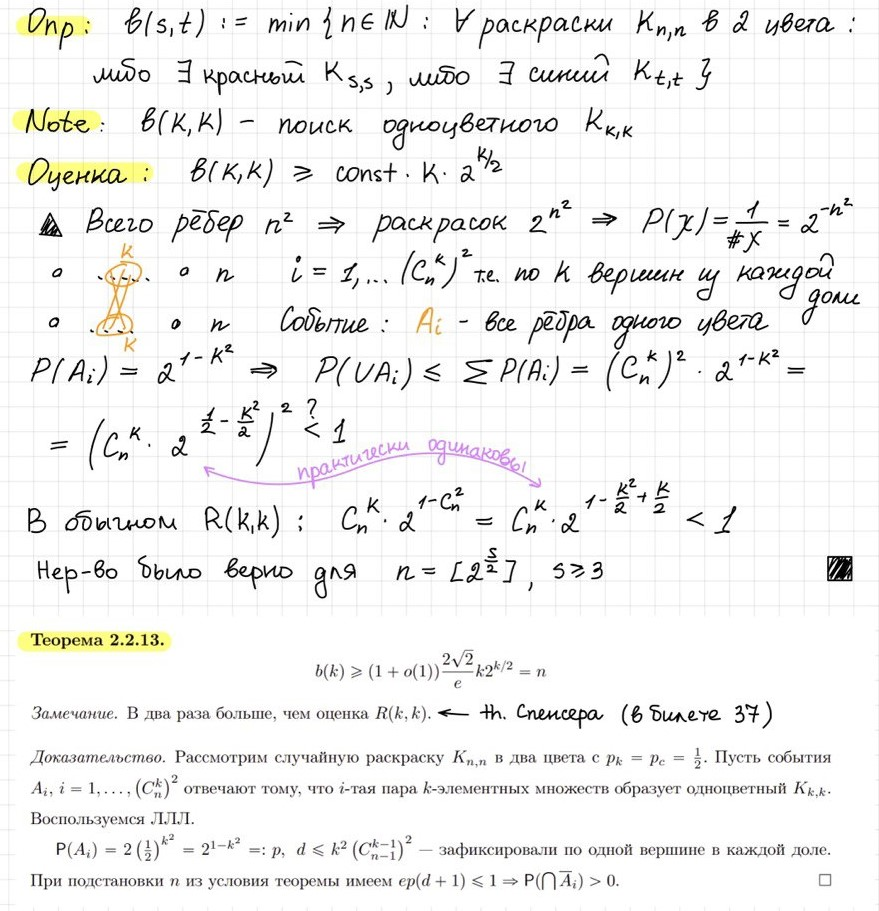
\includegraphics[width=1\linewidth]{sections/Polina/imgs/200.jpg}

% \newpage
\section{Additional information}

\end{document}